% Used in algorithms
\newcommand{\afor}{\textbf{for} {}}
\newcommand{\aif}{\textbf{if} {}}
\newcommand{\aelse}{\textbf{else} {}}
\newcommand{\seq}[1]{\left\langle{#1}\right\rangle}

% Boldface letters
\renewcommand{\AA}{{A}}
\newcommand{\BB}{{B}}
\newcommand{\CC}{{C}}
\newcommand{\FF}{{F}}
\newcommand{\II}{{I}}
\newcommand{\MM}{{M}}
\newcommand{\PP}{{P}}
\renewcommand{\SS}{{S}}
\newcommand{\VV}{{V}}
\newcommand{\bb}{{b}}
\newcommand{\ee}{{e}}

\newcommand{\nn}{{n}}
\newcommand{\uu}{{u}}
\newcommand{\vv}{{v}}
\newcommand{\ww}{{w}}
\newcommand{\xx}{{x}}
\newcommand{\ff}{{f}}

\newcommand{\bpsi}{\bm{\psi}}
\newcommand{\bphi}{\bm{\phi}}
\newcommand{\bPsi}{\bm{\Psi}}
\newcommand{\bPhi}{\bm{\Phi}}

% Caligraphic letters
\newcommand{\mI}{\mathfrak{I}}

\newcommand{\Cc}{\mathcal{C}}
\newcommand{\Dc}{\mathcal{D}}
\newcommand{\Ic}{\mathcal{I}}

\newcommand{\mop}[1]{\operatorname{#1}}
\newcommand{\spans}[1]{\mop{span}\left\{ #1 \right\}}

%//////////////////////////////////////////////////////////////////////////////
\fenicschapter{UFL: a finite element form language}
              {UFL: a finite element form language}
              {Martin Sandve Aln\ae{}s}
              {alnes-1}
%\\\\\\\\\\\\\\\\\\\\\\\\\\\\\\\\\\\\\\\\\\\\\\\\\\\\\\\\\\\\\\\\\\\\\\\\\\\\\\

\index{Unified Form Language}
\index{\ufl{}}
\index{variational form}
\index{weak form}
\index{functional}
\index{form language}
\index{domain specific language}

The Unified Form Language -- \ufl{} \citep{AlnaesLogg2009} --
is a domain specific language for the declaration of finite element
discretizations of variational forms and functionals. More precisely,
the language defines a flexible user interface for defining finite
element spaces and expressions for weak forms in a notation close to
mathematical notation.

The \fenics{} project provides a framework for building applications
for solving partial differential equations (PDEs).  \ufl{} is one of
the core components of this framework.  It defines the language you
\emph{express} your PDEs in.  It is the input language and front-end
of the form compilers \ffc{} and \sfc{}, which are covered in
Chapter~\ref{chap:logg-1} and Chapter~\ref{chap:alnes-3}.  The \ufl{}
implementation also provides algorithms that the form compilers can
use to simplify the compilation process.  The output from these form
compilers is C++ \citep{Stroustrup1997} code that conforms to the \ufc{}
specification, which is explained in Chapter~\ref{chap:alnes-2}.
This code can be used with the C++/Python library \dolfin{}, which
is covered in Chapter~\ref{chap:logg-2}, to efficiently assemble
linear systems and compute solutions to PDEs.  Note that this chapter
does not cover how to actually solve equations defined in UFL. See
Chapter~\ref{chap:langtangen} for a tutorial on how to use the complete
\fenics{} framework to solve equations.

This chapter is intended both for the \fenics{} user who wants
to learn how to express her equations, and for other \fenics{}
developers and technical users who wants to know how \ufl{}
works on the inside.  Therefore, the sections of this chapter
are organized with an increasing amount of technical details.
Sections~\ref{ufl:sec:overview}-\ref{ufl:sec:formtransformations}
give an overview of the language as seen by
the end-user and is intended for all audiences.
Sections~\ref{ufl:sec:representation}-\ref{ufl:sec:implementation}
explain the design of the implementation and dive into some implementation
details.  Many details of the language has to be omitted in a text such
as this, and we refer to the \ufl{} manual \citep{AlnaesLogg2009} for
a more thorough description. Note that this chapter refers to \ufl{}
version 0.5.4, and both the user interface and the implementation may
change in future versions.

Starting with a brief overview, we mention the main design goals
for \ufl{} and show an example implementation of a non-trivial
PDE in Section~\ref{ufl:sec:overview}.  Next we will look at how
to define finite element spaces in Section~\ref{ufl:sec:elements},
followed by the overall structure of forms and their declaration in
Section~\ref{ufl:sec:forms}.  The main part of the language is concerned
with defining expressions from a set of data types and operators, which
are discussed in Section~\ref{ufl:sec:defexpr}.  Operators applying to
entire forms is the topic of Section~\ref{ufl:sec:formtransformations}.

The technical part of the chapter begins with
Section~\ref{ufl:sec:representation} which discusses the
representation of expressions.  Building on the notation and
data structures defined there, how to compute derivatives is
discussed in Section~\ref{ufl:sec:ad}.  Some central internal
algorithms and key issues in their implementation are discussed in
Section~\ref{ufl:sec:algorithms}.  Implementation details, some of which
are specific to the programming language Python \citep{Rossumothers},
is the topic of Section~\ref{ufl:sec:implementation}.  Finally,
Section~\ref{ufl:sec:future} discusses future prospects of the \ufl{}
project.

%------------------------------------------------------------------------------
\subsection{Related work} \label{ufl:sec:related}

The combination of domain specific languages and symbolic computing
with finite element methods has been pursued from other angles in
several other projects.  Sundance \citep{Long2003,Long2004a,Long2004}
implements a symbolic engine directly in C++ to define variational
forms, and has support for automatic differentiation.  The Life
\citep{Prudhomme2006a,Prudhomme2006} project uses a domain specific
language embedded in C++, based on expression template techniques
to specify variational forms.  SfePy \citep{Cimrman2008} uses SymPy
as a symbolic engine, extending it with finite element methods.
GetDP \citep{DularGeuzaine2005} is another project using a domain
specific language for variational forms.  The Mathematica package
AceGen \citep{Korelc1997,Korelc2002} uses the symbolic capabilities
of Mathematica to generate efficient code for finite element methods.
All these packages have in common a focus on high level descriptions
of partial differential equations to achieve higher human efficiency in
the development of simulation software.

\ufl{} almost resembles a library for symbolic computing, but its
scope, goals and priorities are different from generic symbolic
computing projects such as GiNaC \citep{BauerFrinkKreckel2000},
Swiginac \citep{SkavhaugCertik2009} and SymPy \citep{Certikothers2009}.
Intended as a domain specific language and form compiler frontend, \ufl{}
is not suitable for large scale symbolic computing.

%==============================================================================
\section{Overview} \label{ufl:sec:overview}

%------------------------------------------------------------------------------
\subsection{Design goals} \label{ufl:sec:goals}

\ufl{} is a unification, refinement and reimplementation of the
form languages used in previous versions of \ffc{} and \sfc{}.
The development of this language has been motivated by several factors,
the most important being:
\begin{itemize}
  \item A richer form language, especially for expressing nonlinear PDEs.

  \item Automatic differentiation of expressions and forms.

  \item Improving the performance of the form compiler technology to
  handle more complicated equations efficiently.
\end{itemize}
\ufl{} fulfills all these requirements, and by this it represents a major
step forward in the capabilities of the \fenics{} project.

Tensor algebra and index notation support is modeled after the \ffc{}
form language and generalized further. Several nonlinear operators
and functions which only \sfc{} supported before have been included in
the language.  Differentiation of expressions and forms has become an
integrated part of the language, and is much easier to use than the way
these features were implemented in \sfc{} before.  In summary, \ufl{}
combines the best of \ffc{} and \sfc{} in one unified form language and
adds additional capabilities.

The efficiency of code generated by the new generation of form compilers
based on \ufl{} has been verified to match previous form compiler
benchmarks \citep{AlnaesMardal2009b,OelgaardWells2010}.  The form
compilation process is now fast enough to blend into the regular
application build process.  Complicated forms that previously required
too much memory to compile, or took tens of minutes or even hours to
compile, now compiles in seconds with both \sfc{} and \ffc{}.

%------------------------------------------------------------------------------
\subsection{Motivational example}
\label{ufl:sec:example}

One major motivating example during the initial development of \ufl{} has
been the equations for elasticity with large deformations.  In particular,
models of biological tissue use complicated hyperelastic constitutive
laws with anisotropies and strong nonlinearities.  To implement these
equations with \fenics{}, all three design goals listed above had to be
addressed. Below, one version of the hyperelasticity equations and their
corresponding \ufl{} implementation is shown.  Keep in mind that this is
only intended as an illustration of the close correspondence between the
form language and the natural formulation of the equations.  The meaning
of these equations is not necessary for the reader to understand.
Chapter~\ref{chap:narayanan} covers nonlinear elasticity in more detail.
Note that many other examples are distributed together with \ufl{}.

In the formulation of the hyperelasticity equations presented
here, the unknown function is the displacement vector field $\uu$.
The material coefficients $c_1$ and $c_2$ are scalar constants.
The second Piola-Kirchoff stress tensor $\SS$ is computed from the
strain energy function $W(\CC)$. $W$ defines the constitutive law, here
a simple Mooney-Rivlin law. The equations relating the displacement and
stresses read:
\begin{align}
\begin{split}
\FF   &=  \II + \Grad \uu, \\
\CC   &=  \FF^{\top}\FF, \\
I_C   &=  \mop{tr}(\CC), \\
II_C  &=  \frac 1 2 (\mop{tr}(\CC)^2 - \mop{tr}(\CC\CC)), \\
W     &=  c_1(I_C - 3) + c_2(II_C - 3), \\
\SS   &=  2\frac{\partial W}{\partial\CC}.  \label{ufl:eq:hypdef}
\end{split}
\end{align}
For simplicity in this example, we ignore external body and boundary
forces and assume a quasi-stationary situation, leading to the following
mechanics problem. Find $\uu$ such that
\begin{align}
\Div (\FF\SS) &= 0, \quad \mbox{in} \dx, \label{ufl:eq:ppeqzero} \\
\uu &= \uu_0,       \quad \mbox{on} \ds.
\end{align}
The finite element method is presented in Chapter~\ref{chap:kirby-7},
so we will only very briefly cover the steps we take here.  First we
multiply Equation~\eqref{ufl:eq:ppeqzero} with a test function $\bphi
\in V$, then integrate over the domain $\Omega$, and integrate by parts.
The nonlinear variational problem then reads: Find $\uu \in V$ such that
\begin{align}
L(\uu; \bphi) &= \int_\Omega \FF\SS : \Grad\bphi \dx = 0
  \quad \foralls \bphi \in V. \label{ufl:eq:hypdefL}
\end{align}
Here we have omitted the coefficients $c_1$ and $c_2$ for brevity.
Approximating the displacement field as $\uu \approx \uu_h = \sum_k
u_k \bpsi_k$, where $\bpsi_k \in V_h \approx V$ are trial functions,
and using Newtons's method to solve the nonlinear equations, we end up
with a system of equations to solve
\begin{align}
\sum_{k=1}^{|V_h|} \frac{\partial L(\uu_h; \bphi)}{\partial u_k} \Delta u_k =
  -L(\uu_h; \bphi)
  \quad \foralls \bphi \in V_h. \label{ufl:eq:elasticitynewton}
\end{align}
A bilinear form $a(\uu; \bpsi, \bphi)$ corresponding to the left-hand side
of Equation~\eqref{ufl:eq:elasticitynewton} can be computed automatically
by \ufl{}, such that
\begin{align}
a(\uu_h; \bpsi_k, \bphi) = \frac{\partial L(\uu_h; \bphi)}{\partial u_k}
  \quad k = 1, \ldots, |V_h|. \label{alnes-1:eq:hypdefa}
\end{align}

Figure~\ref{ufl:fig:hypcode} shows an implementation of equations
\eqref{ufl:eq:hypdef}, \eqref{ufl:eq:hypdefL} and \eqref{alnes-1:eq:hypdefa}
in \ufl{}.  Notice the close relation between the mathematical notation
and the \ufl{} source code. In particular, note the automated
differentiation of both the constitutive law and the residual
equation. The operator \emp{diff} can be applied to expressions
to differentiate w.r.t designated variables such as \emp{C} here,
while the operator \emp{derivative} can be applied to entire forms
to differentiate w.r.t. each coefficient of a discrete function such
as \emp{u}.  The combination of these features allows a new material
law to be implemented by simply changing $W$, the rest is automatic.
In the following sections, the notation, definitions and operators used
in this implementation will be explained.

\begin{figure}
\begin{uflcode}
# Finite element spaces
cell = tetrahedron
element = VectorElement("CG", cell, 1)

# Form arguments
phi0 = TestFunction(element)
phi1 = TrialFunction(element)
u = Coefficient(element)
c1 = Constant(cell)
c2 = Constant(cell)

# Deformation gradient Fij = dXi/dxj
I = Identity(cell.d)
F = I + grad(u)

# Right Cauchy-Green strain tensor C with invariants
C = variable(F.T*F)
I_C = tr(C)
II_C = (I_C**2 - tr(C*C))/2

# Mooney-Rivlin constitutive law
W = c1*(I_C-3) + c2*(II_C-3)

# Second Piola-Kirchoff stress tensor
S = 2*diff(W, C)

# Weak forms
L = inner(F*S, grad(phi0))*dx
a = derivative(L, u, phi1)
\end{uflcode}
\caption{\ufl{} implementation of hyperelasticity equations with a
Mooney-Rivlin material law.}
\label{ufl:fig:hypcode}
\end{figure}

%==============================================================================
\section{Defining finite element spaces} \label{ufl:sec:elements}
\index{finite element}
\index{finite element space}
\index{Lagrange element}
\index{discontinuous Lagrange element}
\index{\emp{FiniteElement}}
\index{\emp{VectorElement}}
\index{\emp{TensorElement}}
\index{\emp{MixedElement}}
A polygonal cell is defined in \ufl{} by a basic shape, and is declared by
\begin{uflcode}
cell = Cell(shapestring)
\end{uflcode}
\ufl{} defines a set of valid polygonal cell shapes: ``interval'',
``triangle'', ``tetrahedron'', ``quadrilateral'', and ``hexahedron''.
\emp{Cell} objects of all shapes are predefined and can be used
instead by writing
\begin{uflcode}
cell = tetrahedron
\end{uflcode}
In the rest of this chapter, a variable name \emp{cell} will be used
where any cell is a valid argument, to make the examples dimension
independent wherever possible.

\ufl{} defines syntax for \emph{declaring} finite element spaces, but
does not know anything about the actual polynomial basis or degrees of
freedom. The polynomial basis is selected implicitly by choosing among
predefined basic element families and providing a polynomial degree,
but \ufl{} only assumes that there \emph{exists} a basis with a fixed
ordering for each finite element space $V_h$; that is,
\begin{align}
V_h = \spans{\phi_j}_{j=1}^{n}.
\end{align}
Basic scalar elements can be combined to form vector elements or
tensor elements, and elements can easily be combined in arbitrary
mixed element hierarchies.

The set of predefined\footnote{Form compilers can register additional
  element families.}  element family names in \ufl{} includes
``Lagrange'' (short name ``CG''), representing scalar Lagrange finite
elements (continuous piecewise polynomial functions), ``Discontinuous
Lagrange'' (short name ``DG''), representing scalar discontinuous
Lagrange finite elements (discontinuous piecewise polynomial
functions), and a range of other families that can be found in the
manual.  Each family name has an associated short name for
convenience.  To print all valid families to screen from Python, call
\emp{show\_elements()}.

The syntax for declaring elements is best explained with some
examples.
\begin{uflcode}
cell = tetrahedron

P = FiniteElement("Lagrange", cell, 1)
V = VectorElement("Lagrange", cell, 2)
T = TensorElement("DG", cell, 0, symmetry=True)

TH = V * P
ME = MixedElement(T, V, P)
\end{uflcode}
In the first line a polygonal cell is selected from the set of
predefined cells.  Then a scalar linear Lagrange element \emp{P} is
declared, as well as a quadratic vector Lagrange element \emp{V}.
Next a symmetric rank 2 tensor element \emp{T} is defined, which is
also piecewise constant on each cell. The code proceeds to declare a
mixed element \emp{TH}, which combines the quadratic vector element
\emp{V} and the linear scalar element \emp{P}. This element is known
as the Taylor-Hood element.  Finally another mixed element with three
subelements is declared. Note that writing \emp{T * V * P} would not
result in a mixed element with three direct subelements, but rather
\emp{MixedElement(MixedElement(T, V), P)}.

%==============================================================================
\section{Defining forms}
\label{ufl:sec:forms}
\index{\emp{Form}}
\index{\emp{Integral}}
\index{\emp{Measure}}
\index{forms}
\index{integrals}
\index{interior measure}
\index{cell integral}
\index{boundary measure}
\index{exterior facet integral}
\index{boundary measure}
\index{interior facet integral}

Consider Poisson's equation with two different boundary
conditions on $\partial\Omega_0$ and $\partial\Omega_1$,
\begin{align}
a(w; u, v) &= \int_\Omega w \Grad u \cdot \Grad v \dx, \\
L(f, g, h; v) &= \int_\Omega f v \dx + \int_{\partial\Omega_0} g^2 v \ds + \int_{\partial\Omega_1} h v \ds.
\end{align}
These forms can be expressed in UFL as
\begin{uflcode}
a = w*dot(grad(u), grad(v))*dx
L = f*v*dx + g**2*v*ds(0) + h*v*ds(1)
\end{uflcode}
where multiplication by the measures \emp{dx}, \emp{ds(0)} and \emp{ds(1)}
represent the integrals $\int_{\Omega_0} (\cdot) \dx$,
$\int_{\partial\Omega_0} (\cdot) \ds$,
and $\int_{\partial\Omega_1} (\cdot) \ds$
respectively.

Forms expressed in \ufl{} are intended for finite element
discretization followed by compilation to efficient code for computing
the element tensor.  Considering the above example, the bilinear form
$a$ with one coefficient function $w$ is assumed to be evaluated at a
later point with a range of basis functions and the coefficient
function fixed, that is
\begin{align}
V_h^1 &= \spans{\phi_k^1}, \quad V_h^2 = \spans{\phi_k^2}, \quad V_h^3 = \spans{\phi_k^3}, \\
w &= \sum_{k=1}^{|V^3_h|} w_k \phi_k^3, \quad \{ w_k \} \mbox{ given}, \\
A_{ij} &= a(w; \phi_i^1, \phi_j^2),
    \quad i = 1,\ldots,|V^1_h|, \quad j = 1,\ldots,|V^2_h| . \label{ufl:eq:Aij}
\end{align}

In general, \ufl{} is designed to express forms of the following generalized form:
\begin{align} \label{ufl:eq:form_integrals}
    a(w^1, \ldots, w^n; \phi^1, \ldots, \phi^r) =
           \sum_{k=1}^{n_c} \int_{\Omega_k}          I^c_k \dx
         + \sum_{k=1}^{n_e} \int_{\partial\Omega_k}  I^e_k \ds
         + \sum_{k=1}^{n_i} \int_{\Gamma_k}          I^i_k \dS.
\end{align}
Most of this chapter deals with ways to define the integrand
expressions $I^c_k$, $I^e_k$ and $I^i_k$.  The rest of the notation
will be explained below.

The form arguments are divided in two groups, the basis functions
$\phi^1,\ldots,\phi^r$ and the coefficient functions $w^1,\ldots,w^n$.
All $\{ \phi^k \}$ and $\{ w^k \}$ are functions in some discrete
function space with a basis.  Note that the actual basis functions $\{
\phi_j^k \}$ and the coefficients $\{ w_k \}$ are never known to
\ufl{}, but we assume that the ordering of the basis for each finite
element space is fixed. A fixed ordering only matters when
differentiating forms, explained in Section~\ref{ufl:sec:ad}.

Each term of a valid form expression must be a scalar-valued
expression integrated exactly once, and they must be linear in $\{
\phi^k \}$.  Any term may have nonlinear dependencies on coefficient
functions.  A form with one or two basis function arguments ($r=1,2$)
is called a linear or bilinear form respectively, ignoring its
dependency on coefficient functions. These will be assembled to
vectors and matrices when used in an application.  A form depending
only on coefficient functions ($r=0$) is called a functional, since it
will be assembled to a real number. Multilinear forms where $r > 2$
are supported but not as commonly used.

The entire domain is denoted $\Omega$, the external boundary is
denoted $\partial\Omega$, while the set of interior facets of the
triangulation is denoted $\Gamma$. Subdomains are marked with a
suffix, e.g., $\Omega_k \subset \Omega$. As mentioned above,
integration is expressed by multiplication with a measure, and \ufl{}
defines the measures \emp{dx}, \emp{ds} and \emp{dS}.  In
summary, there are three kinds of integrals with corresponding \ufl{}
representations
\begin{itemize}
\item $\int_{        \Omega_k} (\cdot) \dx$ $\leftrightarrow$  $(\cdot)$\emp{*dx(k)}, called a \emph{cell integral},
\item $\int_{\partial\Omega_k} (\cdot) \ds$ $\leftrightarrow$  $(\cdot)$\emp{*ds(k)}, called an \emph{exterior facet integral},
\item $\int_{        \Gamma_k} (\cdot) \dS$ $\leftrightarrow$  $(\cdot)$\emp{*dS(k)}, called an \emph{interior facet integral},
\end{itemize}
Defining a different quadrature order for each term in a form can be
achieved by attaching meta data to measure objects, e.g.,
\begin{uflcode}
dx02 = dx(0, { "integration_order": 2 })
dx14 = dx(1, { "integration_order": 4 })
dx12 = dx(1, { "integration_order": 2 })
L = f*v*dx02 + g*v*dx14 + h*v*dx12
\end{uflcode}
Meta data can also be used to override other form compiler specific
options separately for each term. For more details on this feature see
the manuals of \ufl{} and the form compilers.


%==============================================================================
\section{Defining expressions}
\label{ufl:sec:defexpr}
\index{\emp{Terminal}}
\index{\emp{Identity}}
\index{atomic value}
\index{terminal value}
\index{identity matrix}
\index{spatial coordinates}
\index{facet normal}
\index{form argument}
\index{basis function}
\index{coefficient function}

Most of \ufl{} deals with how to declare expressions such as the
integrand expressions in Equation~\ref{ufl:eq:form_integrals}.  The most
basic expressions are terminal values, which do not depend on other
expressions.  Other expressions are called operators, which are discussed
in sections~\ref{ufl:sec:indexnotation}-\ref{ufl:sec:conditionals}.

Terminal value types in \ufl{} include form arguments (which is the
topic of Section~\ref{ufl:sec:arguments}), geometric quantities, and
literal constants.  Among the literal constants are scalar integer
and floating point values, as well as the $d$ by $d$ identity matrix
\emp{I = Identity(d)}.  To get unit vectors, simply use rows or
columns of the identity matrix, e.g., \emp{e0 = I[0,:]}.  Similarly,
\emp{I[i,j]} represents the Kronecker delta function $\delta_{ij}$
(see Section~\ref{ufl:sec:indexnotation} for details on index
notation).  Available geometric values are the spatial coordinates
$\xx$ $\leftrightarrow$ \emp{cell.x} and the facet normal $\nn$
$\leftrightarrow$ \emp{cell.n}.  The geometric dimension is available
as \emp{cell.d}.

%------------------------------------------------------------------------------
\subsection{Form arguments} \label{ufl:sec:arguments}
\index{form arguments}
\index{functions}
\index{basis functions}
\index{coefficient functions}
\index{coefficients}
\index{\emp{Argument}}
\index{\emp{Arguments}}
\index{\emp{TestFunction}}
\index{\emp{TestFunctions}}
\index{\emp{TrialFunction}}
\index{\emp{TrialFunctions}}
\index{\emp{Coefficient}}
\index{\emp{Coefficients}}
\index{\emp{Constant}}
\index{\emp{VectorConstant}}
\index{\emp{TensorConstant}}
\index{\emp{split}}

Basis functions and coefficient functions are represented by
\emp{Argument} and \emp{Coefficient} respectively. The ordering of the
arguments to a form is decided by the order in which the form arguments
were declared in the \ufl{} code.  Each basis function argument represents
any function in the basis of its finite element space
\begin{align}
  \phi^j \in \{\phi_k^j\}, \quad V_h^j = \spans{\phi_k^j}.
\end{align}
with the intention that the form is later evaluated for all $\phi_k$
such as in Equation~\eqref{ufl:eq:Aij}.  Each coefficient function $w$
represents a discrete function in some finite element space $V_h$; it is
usually a sum of basis functions $\phi_k \in V_h$ with coefficients $w_k$
\begin{align}
w = \sum_{k=1}^{|V_h|} w_k \phi_k.
\end{align}
The exception is coefficient functions that can only be evaluated
point-wise, which are declared with a finite element with family
``Quadrature''.  Basis functions are declared for an arbitrary element
as in the following manner:
\begin{uflcode}
phi = Argument(element)
v = TestFunction(element)
u = TrialFunction(element)
\end{uflcode}
By using \emp{TestFunction} and \emp{TrialFunction} in declarations
instead of \emp{Argument} you can ignore their relative ordering.
The only time \emp{Argument} is needed is for forms of arity $r > 2$.

Coefficient functions are declared similarly for an arbitrary element,
and shorthand notation exists for declaring piecewise constant functions:
\begin{uflcode}
w = Coefficient(element)
c = Constant(cell)
v = VectorConstant(cell)
M = TensorConstant(cell)
\end{uflcode}
If a form argument $u$ in a mixed finite element space $V_h = V_h^0
\times V_h^1$ is desired, but the form is more easily expressed using
subfunctions $u_0 \in V_h^0$ and $u_1 \in V_h^1$, you can split the
mixed function or basis function into its subfunctions in a generic way
using \emp{split}:
\begin{uflcode}
V = V0 * V1
u = Coefficient(V)
u0, u1 = split(u)
\end{uflcode}
The \emp{split} function can handle arbitrary mixed elements.
Alternatively, a handy shorthand notation for argument declaration
followed by \emp{split} is
\begin{uflcode}
v0, v1 = TestFunctions(V)
u0, u1 = TrialFunctions(V)
f0, f1 = Coefficients(V)
\end{uflcode}
%------------------------------------------------------------------------------
\subsection{Index notation}
\label{ufl:sec:indexnotation}
\index{indices}
\index{index notation}
\index{implicit summation}
\index{\emp{Index}}
\index{\emp{indices}}
\index{\emp{IndexSum}}
\index{\emp{Indexed}}
\index{\emp{ComponentTensor}}
\index{\emp{ListTensor}}
\index{\emp{as\_vector}}
\index{\emp{as\_matrix}}
\index{\emp{as\_tensor}}

\ufl{} allows working with tensor expressions of arbitrary rank, using
both tensor algebra and index notation.  A basic familiarity with tensor
algebra and index notation is assumed.  The focus here is on how index
notation is expressed in \ufl{}.

Assuming a standard orthonormal Euclidean basis $\seq{\ee_k}_{k=1}^d$
for $\R^d$, a vector can be expressed with its scalar components in
this basis.  Tensors of rank two can be expressed using their scalar
components in a dyadic basis $\{ \ee_i\otimes\ee_j \}_{i,\,j=1}^d$.
Arbitrary rank tensors can be expressed the same way, as illustrated here.
\begin{align}
\vv &= \sum_{k=1}^{d} v_k \ee_k,
\\
\AA &= \sum_{i=1}^{d} \sum_{j=1}^{d} A_{ij} \ee_i \otimes \ee_j,
\\
\Cc &= \sum_{i=1}^{d} \sum_{j=1}^{d} \sum_k C_{ijk} \ee_i \otimes \ee_j \otimes \ee_k.
\end{align}
Here, $\vv$, $\AA$ and $\Cc$ are rank 1, 2 and 3 tensors respectively.
Indices are called \emph{free} if they have no assigned value, such as
$i$ in $v_i$, and \emph{fixed} if they have a fixed value such as $1$ in
$v_1$. An expression with free indices represents any expression you can
get by assigning fixed values to the indices.  The expression $A_{ij}$ is
scalar valued, and represents any component $(i,j)$ of the tensor $\AA$ in
the Euclidean basis.  When working on paper, it is easy to switch between
tensor notation ($\AA$) and index notation ($A_{ij}$) with the knowledge
that the tensor and its components are different representations of the
same physical quantity.  In a programming language, we must express the
operations mapping from tensor to scalar components and back explicitly.
Mapping from a tensor to its components, for a rank 2 tensor defined as
\begin{equation}
A_{ij} = \AA : (\ee_i\otimes\ee_j)
\end{equation}
is accomplished using indexing with the notation \emp{A[i,j]}.  Defining a
tensor $\AA$ from component values $A_{ij}$ is defined as
\begin{align}
\AA = A_{ij} \ee_i\otimes\ee_j,
\end{align}
and is accomplished using the function \emp{as\_tensor(Aij, (i,j))}.
To illustrate, consider the outer product of two vectors $\AA =
\uu\otimes\vv = u_i v_j \ee_i\otimes\ee_j$, and the corresponding scalar
components $A_{ij}$.  One way to implement this is
\begin{uflcode}
A = outer(u, v)
Aij = A[i, j]
\end{uflcode}
Alternatively, the components of $\AA$ can be expressed directly using
index notation, such as $A_{ij} = u_i v_j$.  $A_{ij}$ can then be mapped
to $\AA$ in the following manner:
\begin{uflcode}
Aij = v[j]*u[i]
A = as_tensor(Aij, (i, j))
\end{uflcode}
These two pairs of lines are mathematically equivalent, and the result
of either pair is that the variable \emp{A} represents the tensor $\AA$
and the variable \emp{Aij} represents the tensor $A_{ij}$.  Note that free
indices have no ordering, so their order of appearance in the expression
\emp{v[j]*u[i]} is insignificant.  Instead of \emp{as\_tensor}, the
specialized functions \emp{as\_vector} and \emp{as\_matrix} can be used.
Although a rank two tensor was used for the examples above, the mappings
generalize to arbitrary rank tensors.

When indexing expressions, fixed indices can also be used such as in
\emp{A[0,1]} which represents a single scalar component.  Fixed
indices can also be mixed with free indices such as in \emp{A[0,i]}.
In addition, slices can be used in place of an index.  An example of
using slices is \emp{A[0,:]} which is a vector expression that
represents row 0 of \emp{A}.  To create new indices, you can either
make a single one or make several at once:
\begin{uflcode}
i = Index()
j, k, l = indices(3)
\end{uflcode}
A set of indices \emp{i}, \emp{j}, \emp{k}, \emp{l} and
\emp{p}, \emp{q}, \emp{r}, \emp{s} are predefined,
and these should suffice for most applications.

If your components are not represented as an expression with free
indices, but as separate unrelated scalar expressions, you can build a
tensor from them using \emp{as\_tensor} and its peers.  As an
example, lets define a 2D rotation matrix and rotate a vector
expression by $\frac \pi 2$:
\begin{uflcode}
th = pi/2
A = as_matrix([[ cos(th), -sin(th)],
               [ sin(th),  cos(th)]])
u = A*v
\end{uflcode}

When indices are repeated in a term, summation over those indices is
implied in accordance with the Einstein convention.  In particular,
indices can be repeated when indexing a tensor of rank two or higher
(\emp{A[i,i]}), when differentiating an expression with a free index
(\emp{v[i].dx(i)}), or when multiplying two expressions with shared
free indices (\emp{u[i]*v[i]}).
\begin{align}
A_{ii}  \equiv \sum_i A_{ii}, \qquad
v_i u_i \equiv \sum_i v_i u_i, \qquad
v_{i,\,i} \equiv \sum_i v_{i,\,i}.
\end{align}

An expression \emp{Aij = A[i,j]} is represented internally using the
\emp{Indexed} class.  \emp{Aij} will reference \emp{A}, keeping the
representation of the original tensor expression \emp{A} unchanged.
Implicit summation is represented explicitly in the expression tree using
the class \emp{IndexSum}.  Many algorithms become easier to implement
with this explicit representation, since e.g. a \emp{Product} instance
can never implicitly represent a sum.  More details on representation
classes are found in Section~\ref{ufl:sec:representation}.

%------------------------------------------------------------------------------
\subsection{Algebraic operators and functions} \label{ufl:sec:algebra}
%\index{+}
%\index{-}
%\index{*}
%\index{/}
%\index{**}
\index{\emp{sin}}
\index{\emp{cos}}
\index{\emp{exp}}
\index{\emp{ln}}
\index{\emp{pow}}
\index{\emp{sqrt}}
\index{dot product}
\index{inner product}
\index{outer product}
\index{cross product}
\index{trace}
\index{determinant}
\index{transpose}
\index{inverse}
\index{language operators}
\index{algebraic operators}
\index{tensor algebra operators}
\index{\emp{dot}}
\index{\emp{inner}}
\index{\emp{outer}}
\index{\emp{cross}}
\index{\emp{tr}}
\index{\emp{det}}
\index{\emp{transpose}}
\index{\emp{inv}}

\ufl{} defines a comprehensive set of operators that can be used for
composing expressions.  The elementary algebraic operators \emp{+},
\emp{-}, \emp{*}, \emp{/} can be used between most \ufl{}
expressions with a few limitations.  Division requires a scalar
expression with no free indices in the denominator.  The operands to a
sum must have the same shape and set of free indices.

The multiplication operator \emp{*} is valid between two scalars, a
scalar and any tensor, a matrix and a vector, and two matrices.  Other
products could have been defined, but for clarity we use tensor
algebra operators and index notation for those rare cases.  A product
of two expressions with shared free indices implies summation over
those indices, see Section~\ref{ufl:sec:indexnotation} for more about
index notation.

Three often used operators are \emp{dot(a, b)}, \emp{inner(a, b)},
and \emp{outer(a, b)}.  The dot product of two tensors of arbitrary
rank is the sum over the last index of the first tensor and the first
index of the second tensor.  Some examples are
\begin{align}
\vv \cdot \uu &= v_i u_i, \\
\AA \cdot \uu &= A_{ij} u_j \ee_i, \\
\AA \cdot \BB &= A_{ik} B_{kj} \ee_i \ee_j, \\
\Cc \cdot \AA &= C_{ijk} A_{kl} \ee_i \ee_j \ee_l.
\end{align}
The inner product is the sum over all indices, for example
\begin{align}
\vv : \uu &= v_i u_i, \\
\AA : \BB &= A_{ij} B_{ij}, \\
\Cc : \Dc &= C_{ijkl} D_{ijkl}.
\end{align}
Some examples of the outer product are
\begin{align}
\vv \otimes \uu &= v_i u_j \ee_i \ee_j, \\
\AA \otimes \uu &= A_{ij} u_k \ee_i \ee_j \ee_k, \\
\AA \otimes \BB &= A_{ij} B_{kl} \ee_i \ee_j \ee_k \ee_l
\end{align}
Other common tensor algebra operators are \emp{cross(u,v)},
\emp{transpose(A)} (or \emp{A.T}), \emp{tr(A)}, \emp{det(A)},
\emp{inv(A)}, \emp{cofac(A)}, \emp{dev(A)}, \emp{skew(A)}, and
\emp{sym(A)}. Most of these tensor algebra operators expect tensors
without free indices. The detailed definitions of these operators are
found in the manual.

A set of common elementary functions operating on scalar expressions
without free indices are included, in particular \emp{abs(f)}, \emp{pow(f,
g)}, \emp{sqrt(f)}, \emp{exp(f)}, \emp{ln(f)}, \emp{sin(f)}, \emp{cos(f)},
and \emp{sign(f)}.

%------------------------------------------------------------------------------
\subsection{Differential operators} \label{ufl:sec:differential}
\index{differential operators}
\index{\emp{Dx}}
\index{\emp{dx}}
\index{\emp{grad}}
\index{\emp{div}}
\index{\emp{curl}}
\index{\emp{rot}}
\index{\emp{diff}}
\index{$\nabla$}

\ufl{} implements derivatives w.r.t. three different kinds of variables.
The most used kind is spatial derivatives.  Expressions can also be
differentiated w.r.t. arbitrary user defined variables.  And the final
kind of derivatives are derivatives of a form or functional w.r.t. the
coefficients of a discrete function; that is, a \emp{Coefficient}
or \emp{Constant}.  Form derivatives are explained in Section
\ref{ufl:sec:derivative}.

Note that derivatives are not computed immediately when declared.
A discussion of how derivatives are computed is found in
Section~\ref{ufl:sec:ad}.

%------------------------------------------------------------------------------
\paragraph{Spatial derivatives}
\label{ufl:sec:dx}

Basic spatial derivatives $\frac{\partial f}{\partial x_i}$ can be
expressed in two equivalent ways:
\begin{uflcode}
df = Dx(f, i)
df = f.dx(i)
\end{uflcode}
Here, \emp{df} represents the derivative of \emp{f} in the spatial
direction $x_i$. The index \emp{i} can either be an integer, representing
differentiation in one fixed spatial direction $x_i$, or an \emp{Index},
representing differentiation in the direction of a free index.
The notation \emp{f.dx(i)} is intended to mirror the index notation
$f_{,i}$, which is shorthand for $\frac{\partial f}{\partial x_i}$.
Repeated indices imply summation, such that the divergence of a vector
valued expression \emp{v} can be written $v_{i,\,i}$, or \emp{v[i].dx(i)}.

Several common compound spatial derivative operators are defined, namely
\emp{div}, \emp{grad}, \emp{curl} and \emp{rot} (rot is a synonym for
curl). Be aware that there are two common ways to define $\mop{grad}$
and $\mop{div}$. Let $s$ be a scalar expression, $\vv$ be a vector
expression, and $\MM$ be a tensor expression of rank $r$.  In \ufl{},
the gradient is then defined as
\begin{align}
\left(\Grad (s) \right)_{i} &= s_{,i}, \\
\left(\Grad (\vv) \right)_{ij} &= v_{i,j}, \\
\left(\Grad (\MM) \right)_{i_1\,\ldots\,i_r\,k} &= M_{i_1\,\ldots\,i_r,\,k},
\end{align}
and the divergence is correspondingly defined as
\begin{align}
\Div (\vv) &= v_{i,\,i}, \\
\left(\Div (\MM) \right)_{i_1\,\ldots\,i_{r-1}} &= M_{i_1\,\ldots\,i_r,\,i_r}.
\end{align}
Thinking in terms of value shape, the gradient appends an axis to the
end of the tensor shape of its operand.  Correspondingly, the divergence
sums over the last index of its operand.

For 3D vector expressions, curl is defined in terms of the nabla operator
and the cross product:
\begin{align}
  \nabla &\equiv \ee_k \frac{\partial}{\partial x_k}, \\
  \mop{curl}(\vv) &\equiv \nabla \times \vv.
\end{align}
For 2D vector and scalar expressions the definitions are:
\begin{align}
  \mop{curl}(\vv) &\equiv v_{1,0} - v_{0,1}, \\
  \mop{curl}(f)   &\equiv f_{,1}\ee_0 - f_{,0}\ee_1.
\end{align}

%------------------------------------------------------------------------------
\paragraph{User defined variables}
\label{ufl:sec:diff}

The second kind of differentiation variables are user-defined
variables, which can represent arbitrary expressions.  Automating
derivatives w.r.t. arbitrary quantities is useful for several tasks, from
differentiation of material laws to computing sensitivities.  An arbitrary
expression $g$ can be assigned to a variable $v$.  An expression $f$
defined as a function of $v$ can be differentiated $f$ w.r.t. $v$:
\begin{align}
v &= g, \\
f &= f(v), \\
h(v) &= \frac{\partial f(v)}{\partial v}.
\end{align}
Setting $g = sin(x_0)$ and $f = e^{v^2}$, gives $h = 2 v e^{v^2} =
2 \sin(x_0) e^{\sin^2(x_0)}$, which can be implemented as follows:
\begin{uflcode}
g = sin(cell.x[0])
v = variable(g)
f = exp(v**2)
h = diff(f, v)
\end{uflcode}
Try running this code in a Python session and print the expressions.
The result is
\begin{python}
>>> print v
var0(sin((x)[0]))
>>> print h
d/d[var0(sin((x)[0]))] (exp((var0(sin((x)[0]))) ** 2))
\end{python}
Note that the variable has a label ``\emp{var0}'', and that \emp{h}
still represents the abstract derivative.  Section~\ref{ufl:sec:ad}
explains how derivatives are computed.

%------------------------------------------------------------------------------
\subsection{Other operators}
\label{ufl:sec:conditionals}
\index{DG operators}
\index{discontinuous Galerkin}
\index{jump}
\index{\emp{jump}}
\index{\emp{avg}}
\index{restriction}

A few operators are provided for the implementation of discontinuous
Galerkin methods.  The basic concept is restricting an expression to
the positive or negative side of an interior facet, which is expressed
simply as \emp{v('+')} or \emp{v('-')} respectively. On top of
this, the operators \emp{avg} and \emp{jump} are implemented,
defined as
\begin{align}
\mop{avg}(v)  &= \frac 1 2 (v^+ + v^-), \\
\mop{jump}(v) &= v^+ - v^- .
\end{align}
These operators can only be used when integrating over the interior facets
(\emp{*dS}).

The only control flow construct included in \ufl{} is conditional
expressions. A conditional expression takes on one of two values depending
on the result of a boolean logic expression. The syntax for this is
\begin{uflcode}
f = conditional(condition, true_value, false_value)
\end{uflcode}
which is interpreted as
\begin{align}
f = \begin{cases}
    t, \quad \mbox{if condition is true}, \\
    f, \quad \mbox{otherwise}.
    \end{cases}
\end{align}
The condition can be one of
%icode{lt(a, b)} $\leftrightarrow$ $(a < b)$,
%icode{gt(a, b)} $\leftrightarrow$ $(a > b)$,
%icode{le(a, b)} $\leftrightarrow$ $(a \le b)$,
%icode{ge(a, b)} $\leftrightarrow$ $(a \ge b)$,
%icode{eq(a, b)} $\leftrightarrow$ $(a = b)$, or
%icode{ne(a, b)} $\leftrightarrow$ $(a \ne b)$.
%\setlength{\columnsep{2in}}
\begin{multicols}{2}
\begin{itemize}
\item \emp{lt(a, b)} $\leftrightarrow$ $(a < b)$
\item \emp{le(a, b)} $\leftrightarrow$ $(a \le b)$
\item \emp{eq(a, b)} $\leftrightarrow$ $(a = b)$
\end{itemize}
\begin{itemize}
\item \emp{gt(a, b)} $\leftrightarrow$ $(a > b)$
\item \emp{ge(a, b)} $\leftrightarrow$ $(a \ge b)$
\item \emp{ne(a, b)} $\leftrightarrow$ $(a \ne b)$
\end{itemize}
\end{multicols}

%==============================================================================
\section{Form operators}
\label{ufl:sec:formtransformations}
\index{form operators}
\index{\emp{action}}
\index{\emp{energy\_norm}}
\index{\emp{lhs}}
\index{\emp{rhs}}
\index{\emp{system}}
\index{\emp{adjoint}}
\index{\emp{replace}}
\index{\emp{derivative}}
\index{\emp{sensitivity\_rhs}}

Once you have defined some forms, there are several ways to compute
related forms from them.  While operators in the previous section are
used to define expressions, the operators discussed in this section are
applied to forms, producing new forms.  Form operators can both make form
definitions more compact and reduce the chances of bugs since changes in
the original form will propagate to forms computed from it automatically.
These form operators can be combined arbitrarily; given a semi-linear
form only a few lines are needed to compute the action of the adjoint
of the Jacobi.  Since these computations are done prior to processing
by the form compilers, there is no overhead at run-time.

%------------------------------------------------------------------------------
\subsection{Differentiating forms}
\label{ufl:sec:derivative}

The form operator \emp{derivative} declares the derivative of a form
w.r.t. coefficients of a discrete function (\emp{Coefficient}).  This
functionality can be used for example to linearize your nonlinear residual
equation (linear form) automatically for use with the Newton-Raphson
method.  It can also be applied multiple times, which is useful to
derive a linear system from a convex functional, in order to find the
function that minimizes the functional.  For non-trivial equations such
expressions can be tedious to calculate by hand.  Other areas in which
this feature can be useful include optimal control and inverse methods,
as well as sensitivity analysis.

In its simplest form, the declaration of the derivative of a form \emp{L}
w.r.t. the coefficients of a function \emp{w} reads
\begin{uflcode}
a = derivative(L, w, u)
\end{uflcode}
The form \emp{a} depends on an additional basis function argument \emp{u},
which must be in the same finite element space as the function \emp{w}.
If the last argument is omitted, a new basis function argument is created.

Let us step through an example of how to apply \emp{derivative} twice
to a functional to derive a linear system.  In the following, $V_h$
is a finite element space with some basis , $w$ is a function in $V_h$,
and $f = f(w)$ is a functional we want to minimize. Derived from $f(w)$
is a linear form $F(w; v)$, and a bilinear form $J(w; u, v)$.
\begin{align}
V_h &= \spans{ \phi_k }, \\
w(x) &= \sum_{k=1}^{|V_h|} w_k \phi_k(x), \\
f&: V_h \rightarrow \R, \\
F(w; \phi_i) &= \frac{\partial f(w)}{\partial w_i},
  \quad i=1,\ldots,|V_h|, \\
J(w; \phi_j, \phi) &= \frac{\partial F(w; \phi)}{\partial w_j},
  \quad j=1,\ldots,|V_h|, \quad \phi\in V_h.
\end{align}
For a concrete functional $f(w) = \int_\Omega \frac 1 2 w^2 \dx$, we
can implement this as
\begin{uflcode}
v = TestFunction(element)
u = TrialFunction(element)
w = Coefficient(element)
f = 0.5 * w**2 * dx
F = derivative(f, w, v)
J = derivative(F, w, u)
\end{uflcode}
This code declares two forms \emp{F} and \emp{J}.  The linear form \emp{F}
represents the standard load vector \emp{w*v*dx} and the bilinear form
\emp{J} represents the mass matrix \emp{u*v*dx}.

Derivatives can also be defined w.r.t. coefficients of a function in a
mixed finite element space.  Consider the Harmonic map equations derived
from the functional
\begin{align} \label{ufl:eq:harmonic}
f(\xx, \lambda) = \int_\Omega \Grad \xx : \Grad \xx + \lambda \xx\cdot\xx \dx,
\end{align}
where $\xx$ is a function in a vector finite element space $V_h^d$
and $\lambda$ is a function in a scalar finite element space
$V_h$.  The linear and bilinear forms derived from the functional in
Equation~\ref{ufl:eq:harmonic} have basis function arguments in the mixed
space $V_h^d \times V_h$. The implementation of these forms with automatic
linearization reads
\begin{uflcode}
Vx = VectorElement("CG", triangle, 1)
Vy = FiniteElement("CG", triangle, 1)
u = Coefficient(Vx * Vy)
x, y = split(u)
f = inner(grad(x), grad(x))*dx + y*dot(x,x)*dx
F = derivative(f, u)
J = derivative(F, u)
\end{uflcode}
Note that the functional is expressed in terms of the subfunctions \emp{x}
and \emp{y}, while the argument to \emp{derivative} must be the single
mixed function \emp{u}.  In this example the basis function arguments
to \emp{derivative} are omitted and thus provided automatically in the
right function spaces.

Note that in computing derivatives of forms, we have assumed that
\begin{align}
\frac{\partial}{\partial w_k} \int_\Omega I \dx
= \int_\Omega \frac{\partial}{\partial w_k} I \dx,
\end{align}
or in particular that the domain $\Omega$ is independent of $w$.
Also, any coefficients other than $w$ are assumed independent of $w$.
Furthermore, note that there is no restriction on the choice of element
in this framework, in particular arbitrary mixed elements are supported.

%------------------------------------------------------------------------------
\subsection{Adjoint}
\label{ufl:sec:adjoint}

Another form operator is the adjoint $a^*$ of a bilinear form $a$,
defined as $a^*(u,v) = a(v,u)$, which is similar to taking the transpose
of the assembled sparse matrix.  In \ufl{} this is implemented simply
by swapping the test and trial functions, and can be written using the
\emp{adjoint} form operator.  An example of its use on an anisotropic
diffusion term looks like
\begin{uflcode}
V = VectorElement("CG", cell, 1)
T = TensorElement("CG", cell, 1)
u = TrialFunction(V)
v = TestFunction(V)
M = Coefficient(T)
a = M[i,j] * u[k].dx(j) * v[k].dx(i) * dx
astar = adjoint(a)
\end{uflcode}
which corresponds to
\begin{align}
a(M; u, v) = \int_\Omega M_{ij} u_{k,j} v_{k,i} \dx, \\
a^*(M; u, v) = a(M; v, u) = \int_\Omega  M_{ij} v_{k,j} u_{k,i} \dx.
\end{align}
This automatic transformation is particularly useful if we need the
adjoint of nonsymmetric bilinear forms computed using
\emp{derivative}, since the explicit expressions for $a$ are not at
hand.  Several of the form operators below are most useful when used
in conjunction with \emp{derivative}.

%------------------------------------------------------------------------------
\subsection{Replacing functions}
\label{ufl:sec:replace}

Evaluating a form with new definitions of form arguments can be done
by replacing terminal objects with other values.  Lets say you have
defined a form \emp{L} that depends on some functions \emp{f} and \emp{g}.
You can then specialize the form by replacing these functions with other
functions or fixed values, such as
\begin{align}
L(f, g; v) = \int_\Omega (f^2 / (2g)) v \dx, \\
L_2(f, g; v) = L(g, 3; v) = \int_\Omega (g^2 / 6) v \dx.
\end{align}
This feature is implemented with \emp{replace}, as illustrated in
this case:
\begin{uflcode}
V = FiniteElement("CG", cell, 1)
v = TestFunction(V)
f = Coefficient(V)
g = Coefficient(V)
L = f**2 / (2*g) * v * dx
L2 = replace(L, { f: g, g: 3})
L3 = g**2 / 6 * v * dx
\end{uflcode}
Here \emp{L2} and \emp{L3} represent exactly the same form. Since they
depend only on \emp{g}, the code generated for these forms can be more
efficient.

%------------------------------------------------------------------------------
\subsection{Action}
\label{ufl:sec:action}

In some applications the matrix is not needed explicitly, only the action
of the matrix on a vector. Assembling the resulting vector directly can be
much more efficient than assembling the sparse matrix and then performing
the matrix-vector multiplication.  Assume \emp{a} is a bilinear form and
\emp{w} is a \emp{Coefficient} defined on the same finite element as
the trial function in \emp{a}.  Let $A$ denote the sparse matrix that
can be assembled from \emp{a}. Then you can assemble the action of $A$
on a vector directly by defining a linear form $L$ representing the
action of a bilinear form $a$ on a function $w$.  The notation for this
is simply \emp{L = action(a, w)}, or even shorter \emp{L = a*w}.
%------------------------------------------------------------------------------
\subsection{Splitting a system}
\label{ufl:sec:system}

If you prefer to write your PDEs with all terms on one side such as
\begin{align}\label{ufl:eq:pde}
a(u, v) - L(v) = 0,
\end{align}
you can declare forms with both linear and bilinear terms and split the
equations into $a$ and $L$ afterwards.  A simple example is
\begin{uflcode}
V = FiniteElement("CG", cell, 1)
u = TrialFunction(V)
v = TestFunction(V)
f = Coefficient(V)
pde = u*v*dx - f*v*dx
a, L = system(pde)
\end{uflcode}
Here \emp{system} is used to split the PDE into its bilinear and
linear parts. Alternatively, \emp{lhs} and \emp{rhs} can be used to
obtain the two parts separately. Make note of the resulting sign of the
linear part, which corresponds to moving $L$ to the right-hand side in
Equation~\eqref{ufl:eq:pde}.

%------------------------------------------------------------------------------
\subsection{Computing the sensitivity of a function} \label{ufl:sec:sensitivity}
% FIXME: Confusing mix of equation above with hypothetical coeff c...
% FIXME: Reviewer found the b/L switching confusing

If you have found the solution $u$ to Equation~\eqref{ufl:eq:pde},
and $u$ depends on some constant scalar value $c$, you can compute the
sensitivity of $u$ w.r.t. changes in $c$.  If $u$ is represented by
a coefficient vector $x$ that is the solution to the algebraic linear
system $A x = b$, the coefficients of $\frac{\partial u}{\partial c}$
are $\frac{\partial x}{\partial c}$.  Applying $\frac{\partial}{\partial
c}$ to $A x = b$ and using the chain rule, we can write
\begin{align}\label{ufl:eq:sL}
A \frac{\partial x}{\partial c} = \frac{\partial b}{\partial c} - \frac{\partial A}{\partial c} x,
\end{align}
and thus $\frac{\partial x}{\partial c}$ can be found by solving the
same algebraic linear system used to compute $x$, only with a different
right-hand side.  The linear form corresponding to the right-hand side
of Equation~\eqref{ufl:eq:sL} can be written
\begin{uflcode}
u = Coefficient(element)
sL = diff(L, c) - action(diff(a, c), u)
\end{uflcode}
or you can use the equivalent form transformation
\begin{uflcode}
sL = sensitivity_rhs(a, u, L, c)
\end{uflcode}
Note that the solution \emp{u} must be represented by a \emp{Coefficient},
while $u$ in $a(u, v)$ is represented by a \emp{Argument}.


%==============================================================================
\section{Expression representation}
\label{ufl:sec:representation}
\index{\emp{Expr}}
\index{\emp{Terminal}}
\index{\emp{Operator}}
\index{terminal value}
\index{operator}
\index{program}
\index{expression}
\index{expression tree}
\index{referential transparency}

From a high level view, \ufl{} is all about defining forms.  Each form
contains one or more scalar integrand expressions, but the form
representation is largely disconnected from the representation of the
integrand expressions.  Indeed, most of the complexity of the \ufl{}
implementation is related to expressing, representing, and manipulating
expressions.  The rest of this chapter will focus on expression
representations and algorithms operating on them.  These topics will
be of little interest to the average user of \ufl{}, and more directed
towards developers and curious technically oriented users.

To reason about expression algorithms without the burden of implementation
details, we need an abstract notation for the structure of an expression.
\ufl{} expressions are representations of programs, and the notation
should allow us to see this connection. Below we will discuss the
properties of expressions both in terms of this abstract notation,
and related to specific implementation details.
%------------------------------------------------------------------------------
\subsection{The structure of an expression}
\label{ufl:sec:expressions}

The most basic expressions, which have no dependencies on other
expressions, are called \emph{terminal expressions}.  Other expressions
result from applying some operator to one or more existing expressions.
Consider an arbitrary (non-terminal) expression $z$.  This expression
depends on a set of terminal expressions $\{ t_i \}$, and is computed
using a set of operators $\{ f_i \}$.  If each subexpression of $z$ is
labeled with an integer, an abstract program can be written to compute
$z$ by computing a sequence of subexpressions $\seq{y_i}_{i=1}^n$ and
setting $z = y_n$.  Algorithm~\ref{ufl:alg:program} shows such a program.

\begin{algorithm}
\afor $i = 1, \ldots, m$:\\
\tab $ y_i =  t_i = \mbox{terminal expression}$ \\
\afor $i = m+1, \ldots, n$:\\
\tab $ y_i =  f_i(\seq{y_j}_{j\in\mI_i})$ \\
$z = y_n$
\caption{Program to compute an expression $z$.}
\label{ufl:alg:program}
\end{algorithm}

Each terminal expression $t_i$ is a literal constant or input argument to
the program. This includes coefficients, basis functions, and geometric
quantities.  A non-terminal subexpression $y_i$ is the result of applying
an operator $f_i$ to a sequence of previously computed expressions
$\seq{y_j}_{j\in\mI_i}$, where $\mI_i$ is an ordered sequence of
expression labels.  Note that the order in which subexpressions
must be computed to produce the same value of $z$ is not unique.
For correctness we only require $j < i \,\, \foralls j \in \mI_i$,
such that all dependencies of a subexpression $y_i$ has been computed
before $y_i$.  In particular, all terminals are numbered first in this
abstract algorithm for notational convenience only.

The program to compute $z$ can be represented as a graph, where each
expression $y_i$ corresponds to a graph vertex. There is a directed
graph edge $e = (i, j)$ from $y_i$ to $y_j$ if $j \in \mI_i$, that is
if $y_i$ depends on the value of $y_j$. More formally, the graph $G$
representing the computation of $z$ consists of a set of vertices $V$
and a set of edges $E$ defined by:
\begin{align}
G &= (V, E), \label{ufl:eq:G} \\
V &= \seq{v_i}_{i=1}^n = \seq{y_i}_{i=1}^n, \label{ufl:eq:V} \\
E &= \{ e_k \} = \bigcup_{i=1}^n \, \left\{ (i, j) \,\, \foralls j \in \mI_i \right\} . \label{ufl:eq:E}
\end{align}
This graph is clearly directed, since dependencies have a direction.
It is acyclic, since an expression can only be constructed from existing
expressions.  Thus a \ufl{} expression can be represented by a directed
acyclic graph (DAG).  There are two ways this DAG can be represented
in \ufl{}. While defining expressions, a linked representation called
the expression tree is built. Technically this is still a DAG since
vertices can be reused in multiple subexpressions, but the representation
emphasizes the tree like structure of the DAG. The other representation
is called the computational graph, which closely mirrors the definition
of $G$ above. This representation is mostly useful for form compilers.
The details of these two DAG representations will be explained below.
They both share the representation of a vertex in the graph as an
expression object, which will be explained next.

%------------------------------------------------------------------------------
\subsection{Expression objects}

\begin{figure}
%\centering
%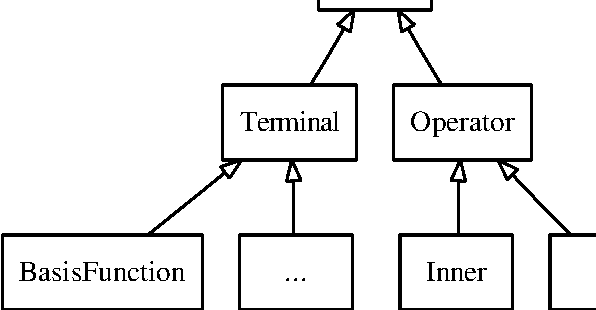
\includegraphics[width=\largefig]{chapters/alnes-1/pdf/expr.pdf}
\def\svgwidth{\largefig}
\import{chapters/alnes-1/pdf/}{expr.pdf_tex}
\caption{Expression class hierarchy.}
\label{ufl:fig:expr}
\end{figure}

Recall from Algorithm~\ref{ufl:alg:program} that non-terminals are
expressions $y_i = f_i(\left<y_j\right>_{j\in\mI_i})$.  The operator
$f_i$ is represented by the class of the expression object, while
the expression $y_i$ is represented by the instance of this class.
In the \ufl{} implementation, each expression object is an instance of
some subclass of \emp{Expr}. The class \emp{Expr} is the superclass of
a hierarchy containing all terminal expression types and operator types
supported by \ufl{}. \emp{Expr} has two direct subclasses, \emp{Terminal}
and \emp{Operator}, which divides the expression type hierarchy in two,
as illustrated in Figure~\ref{ufl:fig:expr}.

All expression objects are considered immutable; once constructed an
expression object will never be modified.  Manipulating an expression
should always result in a new object being created.  The immutable
property ensures that expression objects can be reused and shared
between expressions without side effects in other parts of a program.
This both reduces memory usage, avoids needless copying of objects,
and simplifies recognition of common subexpressions.

Calling \emp{e.operands()} on an \emp{Expr} object \emp{e} representing
$y_i$ returns a tuple with expression objects representing
$\left<y_j\right>_{j\in\mI_i}$.  Note that this also applies to
terminals where there are no outgoing edges and \emp{t.operands()}
returns an empty tuple.  Instead of modifying the operands of an
expression object, a new expression object of the same type can be
constructed with modified operands using \emp{e.reconstruct(operands)},
where \emp{operands} is a tuple of expression objects. If the operands
are the same this function returns the original object, allowing many
algorithms to save memory without additional complications. The invariant
\emp{e.reconstruct(e.operands()) == e} should always hold.


%------------------------------------------------------------------------------
\subsection{Expression properties}

In Section~\ref{ufl:sec:indexnotation} the tensor algebra and index
notation capabilities of \ufl{} was discussed.  Expressions can be
scalar or tensor-valued, with arbitrary rank and shape. Therefore,
each expression object \emp{e} has a value shape \emp{e.shape()},
which is a tuple of integers with the dimensions in each tensor
axis. Scalar expressions have shape \emp{()}. Another important property
is the set of free indices in an expression, obtained as a tuple using
\emp{e.free\_indices()}.  Although the free indices have no ordering, they
are represented with a tuple of \emp{Index} instances for simplicity. Thus
the ordering within the tuple carries no meaning.

\ufl{} expressions are referentially transparent with some
exceptions. Referential transparency means that a subexpression can be
replaced by another representation of its value without changing the
meaning of the expression.  A key point here is that the value of an
expression in this context includes the tensor shape and set of free
indices.  Another important point is that the derivative of a function
$f(v)$ in a point, $f'(v)|_{v=g}$, depends on function values in the
vicinity of $v=g$.  The effect of this dependency is that operator
types matter when differentiating, not only the current value of the
differentiation variable.  In particular, a \emp{Variable} cannot be
replaced by the expression it represents, because \emp{diff} depends on
the \emp{Variable} instance and not the expression it has the value of.
Similarly, replacing a \emp{Coefficient} with some value will change
the meaning of an expression that contains derivatives w.r.t. function
coefficients.

The following example illustrate the issue with \emp{Variable} and
\emp{diff}.
\begin{uflcode}
e = 0
v = variable(e)
f = sin(v)
g = diff(f, v)
\end{uflcode}
Here \emp{v} is a variable that takes on the value 0, but \emp{sin(v)}
cannot be simplified to 0 since the derivative of \emp{f} then would
be 0.  The correct result here is \emp{g = cos(v)}. Printing \emp{f}
and \emp{g} gives the strings \emp{sin(var1(0))} and \emp{d/d[var1(0)]
(sin(var1(0)))}.  Try just setting \emp{v = e} and see how \emp{f}
and \emp{g} becomes zero.

%------------------------------------------------------------------------------
\subsection{Tree representation}

\begin{figure}
%\centering
%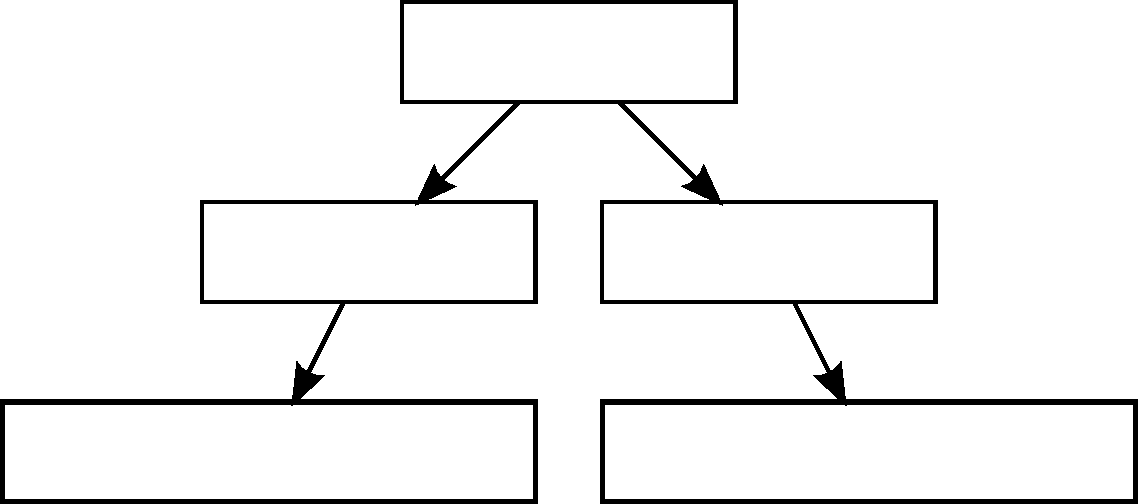
\includegraphics[width=\largefig]{chapters/alnes-1/pdf/stiffness.pdf}
\def\svgwidth{\largefig}
\import{chapters/alnes-1/pdf/}{stiffness.pdf_tex}
\caption{Expression tree for $\Grad \uu : \Grad \vv$.}
\label{ufl:fig:stiffness}
\end{figure}

The expression tree does not have a separate data structure. It is merely
a way of viewing the structure of an expression. Any expression object
\emp{e} can be seen as the root of a tree, where \emp{e.operands()}
returns its children. If some of the children are equal, they will
appear as many times as they appear in the expression. Thus it is easy
to traverse the tree nodes; that is, $v_i$ in the DAG, but eventual
reuse of subexpressions is not directly visible. Edges in the DAG does
not appear explicitly, and the list of vertices can only be obtained by
traversing the tree recursively and selecting unique objects.

An expression tree for the stiffness term $\Grad\uu :\Grad\vv$ is
illustrated in Figure~\ref{ufl:fig:stiffness}.  The terminals $\uu$ and
$\vv$ have no children, and the term $\Grad\uu$ is itself represented by a
tree with two nodes. Each time an operator is applied to some expressions,
it will return a new tree root that references its operands. Note that
the user will apply the functions \emp{grad} and \emp{inner} in her use of
the language, while the names \emp{Grad}, \emp{Inner} and \emp{Argument}
in this figure are the names of the \emp{Expr} subclasses used in \ufl{}
to represent the expression objects.  In other words, taking the gradient
of an expression with \emp{grad(u)} gives an expression representation
\emp{Grad(u)}, and \emp{inner(a, b)} gives an expression representation
\emp{Inner(a, b)}. This separation of language and representation is
merely a design choice in the implementation of \ufl{}.

%------------------------------------------------------------
\subsection{Graph representation} \label{ufl:sec:graphs}
\index{computational graph}

When viewing an expression as a tree, the lists of all unique
vertices and edges are not directly available. Representing the DAG
more directly allows many algorithms to be simplified or optimized.
\ufl{} includes tools to build an array based representation of
the DAG, the \emph{computational graph}, from any expression.
The computational graph $G = V, E$ is a data structure based on
flat arrays, directly mirroring the definition of the graph in
equations~\eqref{ufl:eq:G}-\eqref{ufl:eq:E}.  This representation gives
direct access to dependencies between subexpressions, and allows easy
iteration over unique vertices.  The graph is constructed easily with
the lines:
\begin{python}
from ufl.algorithms import Graph
G = Graph(expression)
V, E = G
\end{python}
One array (Python list)
\emp{V} is used to store the unique vertices $\seq{v_i}_{i=1}^n$ of the
DAG.  For each vertex $v_i$ an expression node $y_i$ is stored to
represent it.  Thus the expression tree for each vertex is also
directly available, since each expression node is the root of its own
expression tree. The edges are stored in an array \emp{E} with
integer tuples \emp{(i,j)} representing an edge from $v_i$ to $v_j$;
that is, $v_j$ is an operand of $v_i$.  The vertex list in the graph
is built using a postordering from a depth first traversal,
which guarantees that the vertices are topologically sorted
such that $j < i \,\, \foralls j \in \mI_i$.

Let us look at an example of a computational graph. The following code
defines a simple expression and then prints the vertices and edges
of its graph.
\begin{python}
from ufl import *
cell = triangle
V = FiniteElement("CG", cell, 1)
u = TrialFunction(V)
v = TestFunction(V)
c = Constant(cell)
f = Coefficient(V)
e = c * f**2 * u * v

from ufl.algorithms import Graph, partition
G = Graph(e)
V, E, = G

print "str(e) = %s\n" % str(e)
print "\n".join("V[%d] = %s" % (i, v) for (i, v) in enumerate(V)), "\n"
print "\n".join("E[%d] = %s" % (i, e) for (i, e) in enumerate(E)), "\n"
\end{python}
An excerpt of the program output is shown here:
\begin{gencode}
V[0] = v_{-2}
...
V[7] = v_{-1} * c_0 * w_1 ** 2
V[8] = v_{-2} * v_{-1} * c_0 * w_1 ** 2
...
E[6] = (8, 0)
E[7] = (8, 7)
\end{gencode}
The two last edges shown here represent the dependencies of vertex 8
on vertex 7 and 0, since $v_8 = v_0 v_7$. Run the code to see the full
output of this code.  Try changing the expression and see what the
graph looks like.

%\begin{gencode}
%str(e) = v_{-2} * v_{-1} * c_0 * w_1 ** 2
%
%V[0] = v_{-2}
%V[1] = v_{-1}
%V[2] = c_0
%V[3] = w_1
%V[4] = 2
%V[5] = w_1 ** 2
%V[6] = c_0 * w_1 ** 2
%V[7] = v_{-1} * c_0 * w_1 ** 2
%V[8] = v_{-2} * v_{-1} * c_0 * w_1 ** 2
%
%E[0] = (5, 3)
%E[1] = (5, 4)
%E[2] = (6, 2)
%E[3] = (6, 5)
%E[4] = (7, 1)
%E[5] = (7, 6)
%E[6] = (8, 0)
%E[7] = (8, 7)
%\end{gencode}

From the edges $E$, related arrays can be computed efficiently; in
particular the vertex indices of dependencies of a vertex $v_i$ in
both directions are useful:
\begin{align}
\begin{split}
V_{out} &= \seq{\mI_i}_{i=1}^{n}, \\
V_{in}  &= \seq{\{ j | i \in \mI_j \}}_{i=1}^{n}
\end{split}
\end{align}
These arrays can be easily constructed for any expression:
\begin{python}
Vin = G.Vin()
Vout = G.Vout()
\end{python}
Similar functions exist for obtaining indices into $E$ for all
incoming and outgoing edges.  A nice property of the computational
graph built by \ufl{} is that no two vertices will represent the same
identical expression.  During graph building, subexpressions are
inserted in a hash map (Python dictionary) to achieve this. Some expression
classes sort their arguments uniquely such that e.g. \emp{a*b} and
\emp{b*a} will become the same vertex in the graph.

Free indices in expression nodes can complicate the interpretation of
the linearized graph when implementing some algorithms, because an
expression object with free indices represents not one value but a set
of values, one for each permutation of the values its free indices can
have.  One solution to this can be to apply \emp{expand\_indices}
before constructing the graph, which will replace all expressions with
free indices with equivalent expressions with explicit fixed indices.
Note however that free indices cannot be regained after expansion.
See Section~\ref{ufl:sec:transformer} for more about this transformation.

%------------------------------------------------------------
\subsection{Partitioning}

\ufl{} is intended as a front-end for form compilers.  Since the
end goal is generation of code from expressions, some utilities are
provided for the code generation process. In principle, correct code
can be generated for an expression from its computational graph simply
by iterating over the vertices and generating code for each operation
separately, basically mirroring Algorithm~\ref{ufl:alg:program}.
However, a good form compiler should be able to produce better code.
\ufl{} provides utilities for partitioning the computational graph into
subgraphs (partitions) based on dependencies of subexpressions, which
enables quadrature based form compilers to easily place subexpressions
inside the right sets of loops.  The function \emp{partition} implements
this feature.  Each partition is represented by a simple array of vertex
indices, and each partition is labeled with a set of dependencies. By
default, this set of dependencies use the strings 'x', 'c', and 'v\%d'
to denote dependencies on spatial coordinates, cell specific quantities,
and form arguments (not coefficients) respectively.

The following example code partitions the graph built above, and prints
vertices in groups based on their dependencies.
\begin{python}
partitions, keys = partition(G)
for deps in sorted(partitions.keys()):
    P = partitions[deps]
    print "The following depends on", tuple(deps)
    for i in sorted(P):
        print "V[%d] = %s" % (i, V[i])
\end{python}
The output text from the program is included below.  Notice that the
literal constant 2 has no dependencies. Expressions in this partition can
always be precomputed compile-time. The \emp{Constant} \emp{c\_0} depends
on data which varies for each cell, represented by 'c' in the dependency
set, but not on spatial coordinates, so it can be placed outside the
quadrature loop. The \emp{Function} \emp{w\_1} and expressions depending
on it depends in addition on the spatial coordinates, represented by
'x', and therefore needs to be computed for each quadrature point.
Expressions depending on only the test or trial function are marked
with 'v\%d' where the number is the internal counter used by \ufl{} to
distinguish between arguments.  Note that test and trial functions are
here marked as depending on the spatial coordinates, but not on cell
dependent quantities. This is only true for finite elements defined
on a local reference element, in which case the basis functions can be
precomputed in each quadrature point.  The actual run-time dependencies
of a basis function in a finite element space is unknown to \ufl{},
which is why the partition function takes an optional multifunction
argument such that the form compiler writer can provide more accurate
dependencies. We refer to the implementation of \emp{partition} for such
implementation details.
\begin{gencode}
The following depends on ()
V[4] = 2
The following depends on ('c',)
V[2] = c_0
The following depends on ('x', 'c')
V[3] = w_1
V[5] = w_1 ** 2
V[6] = c_0 * w_1 ** 2
The following depends on ('x', 'v-1')
V[1] = v_{-1}
The following depends on ('x', 'c', 'v-1')
V[7] = v_{-1} * c_0 * w_1 ** 2
The following depends on ('x', 'v-2')
V[0] = v_{-2}
The following depends on ('x', 'c', 'v-2', 'v-1')
V[8] = v_{-2} * v_{-1} * c_0 * w_1 ** 2
\end{gencode}

%==============================================================================
\section{Computing derivatives} \label{ufl:sec:ad}
\index{computing derivatives}
\index{Automatic Differentiation}
\index{AD}
\index{forward mode AD}
\index{reverse mode AD}
\index{symbolic differentiation}
\index{differentiation}
\index{derivatives}

When any kind of derivative expression is declared by the end-user of
the form language, an expression object is constructed to represent
it, but nothing is computed.  The type of this expression object is a
subclass of \emp{Derivative}. Before low level code can be generated
from the derivative expression, some kind of algorithm to evaluate
derivatives must be applied, since differential operators are not
available natively in low level languages such as C++.  Computing exact
derivatives is important, which rules out approximations by divided
differences.  Several alternative algorithms exist for computing exact
derivatives.  All relevant algorithms are based on the chain rule
combined with differentiation rules for each expression object type.
The main differences between the algorithms are in the extent of which
subexpressions are reused, and in the way subexpressions are accumulated.

Mixing derivative computation into the code generation strategy
of each form compiler would lead to a significant duplication of
implementation effort.  To separate concerns and keep the code manageable,
differentiation is implemented as part of \ufl{} in such a way that the
form compilers are independent of the differentiation strategy chosen in
\ufl{}. Therefore, it is advantageous to use the same representation for
the evaluated derivative expressions as for any other expression. Before
expressions are interpreted by a form compiler, differential operators
should be evaluated such that the only operators left are non-differential
operators. An exception is made for spatial derivatives of terminals which
are unknown to \ufl{} because they are provided by the form compilers.

Below, the differences and similarities between some of the simplest
algorithms are discussed.  After the algorithm currently implemented
in \ufl{} has been explained, extensions to tensor and index notation
and higher order derivatives are discussed.  Finally, the section is
closed with some remarks about the differentiation rules for terminal
expressions.
%------------------------------------------------------------
\subsection{Approaches to computing derivatives}
\label{ufl:sec:appcompder}

Algorithms for computing derivatives are designed with different end goals
in mind.  Symbolic Differentiation (SD) takes as input a single symbolic
expression and produces a new symbolic expression for its derivative.
Automatic Differentiation (AD) takes as input a program to compute
a function and produces a new program to compute the derivative of
the function.  Several variants of AD algorithms exist, the two most
common being Forward Mode AD and Reverse Mode AD \citep{Griewank1989}.
More advanced algorithms exist, and is an active research topic. A
\ufl{} expression is a symbolic expression, represented by an expression
tree. But the expression tree is a directed acyclic graph that represents
a program to evaluate said expression.  Thus it seems the line between
SD and AD becomes less distinct in this context.

Naively applied, SD can result in huge expressions, which can both require
a lot of memory during the computation and be highly inefficient if
written to code directly. However, some illustrations of the inefficiency
of symbolic differentiation, such as in \citet{Griewank1989}, are based
on computing closed form expressions of derivatives in some stand-alone
computer algebra system (CAS).  Copying the resulting large expressions
directly into a computer code can lead to very inefficient code. The
compiler may not be able to detect common subexpressions, in particular
if simplification and rewriting rules in the CAS has changed the structure
of subexpressions with a potential for reuse.

In general, AD is capable of handling algorithms that SD can not.  A tool
for applying AD to a generic source code must handle many complications
such as subroutines, global variables, arbitrary loops and branches
\citep{BischofCarleCorlissEtAl1992,BischofHovlandNorris2002,GieringKaminski1998}.
Since the support for program flow constructs in \ufl{} is very limited,
the AD implementation in \ufl{} will not run into such complications.
In Section~\ref{ufl:sec:forwardad} the similarity between SD and forward
mode AD in the context of \ufl{} is explained in more detail.

%------------------------------------------------------------
\subsection{Forward mode automatic differentiation}
\label{ufl:sec:forwardad}

Recall Algorithm~\ref{ufl:alg:program}, which represents a program for
computing an expression $z$ from a set of terminal values $\{ t_i \}$
and a set of elementary operations $\{ f_i \}$. Assume for a moment that
there are no differential operators among $\{ f_i \}$.  The algorithm
can then be extended to compute the derivative $\frac{d z}{d
  v}$, where $v$ represents a differentiation variable of any kind.
This extension gives Algorithm~\ref{ufl:alg:forwardad}.

\begin{algorithm}
\afor $i = 1, \ldots, m$:\\
\tab $y_i = t_i$ \\
\tab $\frac{d y_i}{d v} = \frac{d t_i}{d v}$ \\
\afor $i = m+1, \ldots, n$:\\
\tab $y_i = f_i(\seq{y_j}_{j\in\mI_i})$ \\
\tab $\frac{d y_i}{d v} = \sum_{k\in\mI_i} \frac{\partial f_i}{\partial y_k} \frac{d y_k}{d v}$ \\
$z = y_n$ \\
$\frac{d z}{d v} = \frac{d y_n}{d v}$
\caption{Forward mode AD on Algorithm~\ref{ufl:alg:program}.}
\label{ufl:alg:forwardad}
\end{algorithm}

This way of extending a program to simultaneously compute the expression
$z$ and its derivative $\frac{d z}{d v}$ is called forward mode automatic
differentiation (AD).  By renaming $y_i$ and $\frac{d
  y_i}{d v}$ to a new sequence of values $\seq{\hat y_j}_{j=1}^{\hat n}$,
  Algorithm~\ref{ufl:alg:forwardad} can be rewritten as shown in
Algorithm~\ref{ufl:alg:forwardadprogram}, which is isomorphic to
Algorithm~\ref{ufl:alg:program} (they have exactly the same structure).
\begin{algorithm}
\afor $i = 1, \ldots, \hat m$:\\
\tab $\hat y_i = \hat t_i$ \\
\afor $i = \hat m + 1, \ldots, \hat n$:\\
\tab $\hat y_i = \hat f_i(\seq{\hat y_j}_{j\in\hat\mI_i})$ \\
$\frac{d z}{d v} = \hat y_{\hat n}$
\caption{Program to compute $\frac{d z}{d v}$ produced by forward mode AD}
\label{ufl:alg:forwardadprogram}
\end{algorithm}

Since the program in Algorithm~\ref{ufl:alg:program} can be
represented as a DAG, and Algorithm~\ref{ufl:alg:forwardadprogram}
is isomorphic to Algorithm~\ref{ufl:alg:program}, the program in
Algorithm~\ref{ufl:alg:forwardadprogram} can also be represented as a DAG.
Thus a program to compute $\frac{d z}{d v}$ can be represented by an
expression tree built from terminal values and non-differential operators.

The currently implemented algorithm for computing derivatives in \ufl{}
follows forward mode AD closely. Since the result is a new expression
tree, the algorithm can also be called symbolic differentiation. In this
context, the differences between the two are implementation details.
To ensure that we can reuse expressions properly, simplification rules in
\ufl{} avoids modifying the operands of an operator.  Naturally repeated
patterns in the expression can therefore be detected easily by the
form compilers.  Efficient common subexpression elimination can then
be implemented by placing subexpressions in a hash map.  However, there
are simplifications such as $0*f\rightarrow 0$ and $1*f\rightarrow f$,
called constant folding, which simplify the result of the differentiation
algorithm automatically as it is being constructed.  These simplifications
are crucial for the memory use during derivative computations, and the
performance of the resulting program.
%------------------------------------------------------------
\subsection{Extensions to tensors and indexed expressions}

So far we have not considered derivatives of non-scalar expression and
expressions with free indices.  This issue does not affect the overall
algorithms, but it does affect the local derivative rules for each
expression type.

Consider the expression \emp{diff(A, B)} with \emp{A} and \emp{B} matrix
expressions.  The meaning of derivatives of tensors w.r.t. to tensors
is easily defined via index notation, which is heavily used within the
differentiation rules:
\begin{align}
\frac{d\AA}{d\BB} = \frac{dA_{ij}}{d B_{kl}} \ee_i\otimes\ee_j\otimes\ee_k\otimes\ee_l
\end{align}

Derivatives of subexpressions are frequently evaluated to literal
constants.  For indexed expressions, it is important that free indices
are propagated correctly with the derivatives.  Therefore, differentiated
expressions will some times include literal constants annotated with
free indices.

There is one rare and tricky corner case when an index sum binds an index
$i$ such as in $(v_i v_i)$ and the derivative w.r.t. $x_i$ is attempted.
The simplest example of this is the expression $(v_i v_i)_{,j}$, which has
one free index $j$.  If $j$ is replaced by $i$, the expression can still
be well defined, but you would never write $(v_i v_i)_{,i}$ manually.
If the expression in the parenthesis is defined in a variable \emp{e
= v[i]*v[i]}, the expression \emp{e.dx(i)} looks innocent. However,
this will cause problems as derivatives (including the index $i$) are
propagated up to terminals.  If this case is encountered in the current
implementation of \ufl{}, it will be detected and an error message will
be triggered.  To work around the problem, simply use different index
instances.  In a future version of \ufl{}, this case may be handled by
relabeling indices to change any expression $(\sum_i e_i)_{,i}$ into
$(\sum_j e_j)_{,i}$.

%------------------------------------------------------------
\subsection{Higher order derivatives}

A simple forward mode AD implementation such as
Algorithm~\ref{ufl:alg:forwardad} only considers one differentiation
variable.  Higher order or nested differential operators must also be
supported, with any combination of differentiation variables.  A simple
example illustrating such an expression can be
\begin{align} \label{ufl:eq:nested}
a = \frac{d}{dx}\left( \frac{d}{dx} f(x) + 2 \frac{d}{dy} g(x,y) \right) .
\end{align}
Considerations for implementations of nested derivatives
in a functional\footnote{Functional as in functional
languages.} framework have been explored in several papers
\citep{Karczmarczuk2001,PearlmutterSiskind2007,SiskindPearlmutter2008}.

In the current \ufl{} implementation this is solved in a different
fashion.  Considering Equation~\eqref{ufl:eq:nested}, the approach is
simply to compute the innermost derivatives $\frac{d}{dx} f(x)$ and
$\frac{d}{dy} g(x,y)$ first, and then computing the outer derivatives.
This approach is possible because the result of a derivative computation
is represented as an expression tree just as any other expression.
Mainly this approach was chosen because it is simple to implement
and easy to verify.  Whether other approaches are faster has not been
investigated.  Furthermore, alternative AD algorithms such as reverse
mode can be experimented with in the future without concern for nested
derivatives in the first implementations.

An outer controller function \emp{apply\_ad} handles the application
of a single variable AD routine to an expression with possibly nested
derivatives.  The AD routine is a function accepting a derivative
expression node and returning an expression where the single variable
derivative has been computed.  This routine can be an implementation of
Algorithm~\ref{ufl:alg:forwardadprogram}.  The result of \emp{apply\_ad}
is mathematically equivalent to the input, but with no derivative
expression nodes left\footnote{Except direct spatial
  derivatives of form arguments, but that is an implementation detail.}.

The function \emp{apply\_ad} works by traversing the tree recursively
in post-order, discovering subtrees where the root represents a
derivative, and applying the provided AD routine to the derivative
subtree.  Since the children of the derivative node has already
been visited by \emp{apply\_ad}, they are guaranteed to be free of
derivative expression nodes and the AD routine only needs to handle
the case discussed above with algorithms \ref{ufl:alg:forwardad} and
\ref{ufl:alg:forwardadprogram}.

The complexity of the \emp{ad\_routine} should be $O(n)$, with $n$
being the size of the expression tree.  The size of the derivative
expression is proportional to the original expression.  If there are
$d$ derivative expression nodes in the expression tree, the complexity
of this algorithm is $O(d n)$, since \emp{ad\_routine} is applied to
subexpressions $d$ times.  As a result the worst case complexity of
\emp{apply\_ad} is $O(n^2)$, but in practice $d \ll n$.  A recursive
implementation of this algorithm is shown in Figure~\ref{ufl:fig:applyad}.

\begin{figure}
\begin{python}
def apply_ad(e, ad_routine):
    if isinstance(e, Terminal):
        return e
    ops = [apply_ad(o, ad_routine) for o in e.operands()]
    e = e.reconstruct(*ops)
    if isinstance(e, Derivative):
        e = ad_routine(e)
    return e
\end{python}
\caption{Simple implementation of recursive \emp{apply\_ad} procedure.}
\label{ufl:fig:applyad}
\end{figure}

%------------------------------------------------------------
\subsection{Basic differentiation rules}

To implement the algorithm descriptions above, we must implement
differentiation rules for all expression node types. Derivatives
of operators can be implemented as generic rules independent of the
differentiation variable, and these are well known and not mentioned
here. Derivatives of terminals depend on the differentiation variable
type.  Derivatives of literal constants are of course always zero,
and only spatial derivatives of geometric quantities are nonzero.
Since form arguments are unknown to \ufl{} (they are provided externally
by the form compilers), their spatial derivatives ($\frac{\partial
  \phi^k}{\partial x_i}$ and $\frac{\partial w^k}{\partial x_i}$) are
considered input arguments as well.  In all derivative computations,
the assumption is made that form coefficients have no dependencies
on the differentiation variable.  Two more cases needs explaining,
the user defined variables and derivatives w.r.t. the coefficients of
a \texttt{Coefficient}.

If $v$ is a \emp{Variable}, then we define $\frac{d t}{d v} \equiv 0$
for any terminal $t$. If $v$ is scalar valued then $\frac{d v}{d v}
\equiv 1$. Furthermore, if $\VV$ is a tensor valued \emp{Variable},
its derivative w.r.t. itself is
\begin{align}
\frac{d \VV}{d \VV}
    =
    \frac{d V_{ij}}{d V_{kl}}
    \ee_i\otimes\ee_j\otimes\ee_k\otimes\ee_l
    =
    \delta_{ik}\delta_{jl}
    \ee_i\otimes\ee_j\otimes\ee_k\otimes\ee_l .
\end{align}
In addition, the derivative of a variable w.r.t. something else than
itself equals the derivative of the expression it represents:
\begin{align}
v &= g, \\
\frac{d v}{d z} &= \frac{d g}{d z}.
\end{align}

Finally, we consider the operator \emp{derivative}, which represents
differentiation w.r.t. all coefficients $\{w_k\}$ of a function $w$.
Consider an object \emp{element} which represents a finite element space
$V_h$ with a basis $\{\phi_k\}$.  Next consider form arguments defined
in this space:
\begin{uflcode}
v = Argument(element)
w = Coefficient(element)
\end{uflcode}
The Argument instance \emp{v} represents any $v\in\{\phi_k\}$,
while the \emp{Coefficient} instance \emp{w} represents the sum
\begin{align}
w = \sum_k w_k \phi_k(x).
\end{align}
The derivative of \emp{w} w.r.t. any $w_k$ is the corresponding basis
function in $V_h$,
\begin{align}
\frac{\partial w}{\partial w_k} = \phi_k, \quad k = 1, \ldots, |V_h|, \\
\end{align}
which can be represented by \emp{v}, since
\begin{align}
v \in \seq{ \phi_k }_{k=1}^{|V_h|} = \seq{ \frac{\partial w}{\partial w_k} }_{k=1}^{|V_h|}.
\end{align}
Note that \emp{v} should be a basis function instance that has not
already been used in the form.

%==============================================================================
\section{Algorithms}
\label{ufl:sec:algorithms}
\index{algorithms}

In this section, some central algorithms and key implementation issues
are discussed, much of which relates to the Python programming language.
Thus, this section is mainly intended for developers and others who need
to relate to \ufl{} on a technical level.  Python users may also find
some of the techniques here interesting.

%------------------------------------------------------------
\subsection{Effective tree traversal in Python}
\label{ufl:sec:traversal}

\index{expression trees}
\index{tree traversal}

Applying some action to all nodes in a tree is naturally expressed
using recursion:
\begin{python}
def walk(expression, pre_action, post_action):
    pre_action(expression)
    for o in expression.operands():
        walk(o)
    post_action(expression)
\end{python}
This implementation simultaneously covers pre-order traversal, where
each node is visited before its children, and post-order traversal,
where each node is visited after its children.

A more ``pythonic'' way to implement iteration over a collection of
nodes is using generators.  A minimal implementation of this could be
\begin{python}
def post_traversal(root):
    for o in root.operands():
        yield post_traversal(o)
    yield root
\end{python}
which then enables the natural Python syntax for iteration over expression
nodes:
\begin{python}
for e in post_traversal(expression):
    post_action(e)
\end{python}
For efficiency, the actual implementation of \emp{post\_traversal}
in \ufl{} is not using recursion.  Function calls are very expensive
in Python, which makes the non-recursive implementation an order of
magnitude faster than the above.

%------------------------------------------------------------
\subsection{Type based function dispatch in Python}
\label{ufl:sec:multifunction}
\index{multifunctions}

A common task in both symbolic computing and compiler implementation
is the selection of some operation based on the type of an expression
node.  For a selected few operations, this is done using overloading
of functions in the subclasses of \emp{Expr}, but this is not suitable
for all operations.  In many cases type-specific operations are better
implemented together in the algorithm instead of distributed across
class definitions.  This implementation pattern is called the Visitor
pattern \citep{GammaHelmJohnsonEtAl1995}.  The implementation in \ufl{}
is somewhat different from the patterns used in a statically typed
language such as C++.

One way to implement type based operation selection is to use a type
switch, or a sequence of if-tests such as this:
\begin{python}
if isinstance(expression, IntValue):
    result = int_operation(expression)
elif isinstance(expression, Sum):
    result = sum_operation(expression)
# etc.
\end{python}
There are several problems with this approach, one of which is
efficiency when there are many types to check.  A type based function
dispatch mechanism with efficiency independent of the number of types
is implemented as an alternative through the class \emp{MultiFunction}.
The underlying mechanism is a dictionary lookup (which is $O(1)$) based on
the type of the input argument, followed by a call to the function found
in the dictionary. The lookup table is built in the \emp{MultiFunction}
constructor only once.  Functions to insert in the table are discovered
automatically using the introspection capabilities of Python.

A multifunction is declared as a subclass of \emp{MultiFunction}. For each
type that should be handled particularly, a member function is declared
in the subclass.  The \emp{Expr} classes use the \emp{CamelCaps} naming
convention, which is automatically converted to \emp{underscore\_notation}
for corresponding function names, such as \emp{IndexSum} and
\emp{index\_sum}.  If a handler function is not declared for a type,
the closest superclass handler function is used instead.  Note that
the \emp{MultiFunction} implementation is specialized to types in the
\emp{Expr} class hierarchy.  The declaration and use of a multifunction
is illustrated in Figure~\ref{ufl:fig:examplefunction}.  Note that
\emp{argument} and \emp{sum} will handle instances of the exact types
\emp{Argument} and \emp{Sum}, while \emp{terminal} and \emp{operator}
will handle the types \emp{SpatialCoordinate} and \emp{Product} since
they have no specific handlers.

\begin{figure}
\begin{python}
class ExampleFunction(MultiFunction):
    def __init__(self):
        MultiFunction.__init__(self)

    def terminal(self, expression):
        return "Got a Terminal subtype %s." % type(expression)

    def operator(self, expression):
        return "Got an Operator subtype %s." % type(expression)

    def argument(self, expression):
        return "Got an Argument."

    def sum(self, expression):
        return "Got a Sum."

m = ExampleFunction()

cell = triangle
element = FiniteElement("CG", cell, 1)
x = cell.x
print m(Argument(element))
print m(x)
print m(x[0] + x[1])
print m(x[0] * x[1])
\end{python}
\caption{Example declaration and use of a multifunction.}
\label{ufl:fig:examplefunction}
\end{figure}
%------------------------------------------------------------
\subsection{Implementing expression transformations}
\label{ufl:sec:transformer}
\index{expression transformations}

Many transformations of expressions can be implemented recursively with
some type-specific operation applied to each expression node.  Examples of
operations are converting an expression node to a string representation,
to an expression representation using an symbolic external library, or
to a \ufl{} representation with some different properties.  A simple
variant of this pattern can be implemented using a multifunction to
represent the type-specific operation:
\begin{python}
def apply(e, multifunction):
    ops = [apply(o, multifunction) for o in e.operands()]
    return multifunction(e, *ops)
\end{python}
The basic idea is as follows. Given an expression node \emp{e}, begin
with applying the transformation to each child node.  Then return the
result of some operation specialized according to the type of \emp{e},
using the already transformed children as input.

The \emp{Transformer} class implements this pattern.  Defining a new
algorithm using this pattern involves declaring a \emp{Transformer}
subclass, and implementing the type specific operations as member
functions of this class just as with \emp{MultiFunction}.  The difference
is that member functions take one additional argument for each operand
of the expression node. The transformed child nodes are supplied as these
additional arguments.  The following code replaces terminal objects with
objects found in a dictionary \emp{mapping}, and reconstructs operators
with the transformed expression trees. The algorithm is applied to an
expression by calling the function \emp{visit}, named after the similar
Visitor pattern.
\begin{python}
class Replacer(Transformer):
    def __init__(self, mapping):
        Transformer.__init__(self)
        self.mapping = mapping

    def operator(self, e, *ops):
        return e.reconstruct(*ops)

    def terminal(self, e):
        return self.mapping.get(e, e)

f = Constant(triangle)
r = Replacer({f: f**2})
g = r.visit(2*f)
\end{python}
After running this code the result is $g = 2 f^2$.  The actual
implementation of the \emp{replace} function is similar to this code.

In some cases, child nodes should not be visited before their parent
node. This distinction is easily expressed using \emp{Transformer},
simply by omitting the member function arguments for the transformed
operands. See the source code for many examples of algorithms using
this pattern.

%------------------------------------------------------------
\subsection{Important transformations} \label{ufl:sec:expanding}
\index{expression transformations}
\index{expression representations}

There are many ways in which expression representations can
be manipulated.  Here, we describe three particularly important
transformations.  Note that each of these algorithms removes some
abstractions, and hence may remove some opportunities for analysis or
optimization. To demonstrate their effect, each transformation will be
applied below to the expression
\begin{align} \label{ufl:eq:a_before_expand}
a   &= \Grad (f u) \cdot \Grad v.
\end{align}
At the end of the section, some example code is given to demonstrate
more representation details.

Some operators in \ufl{} are termed ``compound'' operators, meaning they
can be represented by other more elementary operators.  Try defining an
expression \emp{a = dot(grad(f*u), grad(v))}, and print \emp{repr(a)}. As
you will see, the representation of \emp{a} is \emp{Dot(Grad(Product(f,
u)), Grad(v))}, with some more details in place of \emp{f}, \emp{u}
and \emp{v}.  By representing the gradient directly with a high level
type \emp{Grad} instead of more low level types, the input expressions are
easier to recognize in the representation, and rendering of expressions to
for example \LaTeX{} format can show the original compound operators as
written by the end-user.  However, since many algorithms must implement
actions for each operator type, the function \emp{expand\_compounds} is
used to replace all expression nodes of ``compound'' types with equivalent
expressions using basic types. When this operation is applied to the input
forms from the user, algorithms in both \ufl{} and the form compilers
can still be written purely in terms of more basic operators.  Expanding
the compound expressions from Equation~\eqref{ufl:eq:a_before_expand}
results in the expression
\begin{align} \label{ufl:eq:a_after_expand_compounds}
a_c &= \sum_i \frac{\partial v}{\partial x_i} \frac{\partial (u f)}{\partial x_i}.
\end{align}

Another important transformation is \emp{expand\_derivatives}, which
applies automatic differentiation to expressions, recursively and for
all kinds of derivatives.  The end result is that most derivatives are
evaluated, and the only derivative operator types left in the expression
tree applies to terminals. The precondition for this algorithm is that
\emp{expand\_compounds} has been applied.  Expanding the derivatives in
$a_c$ from Equation~\eqref{ufl:eq:a_after_expand_compounds} gives us
\begin{align} \label{ufl:eq:a_after_expand_derivatives}
a_d &= \sum_{i} \frac{\partial v}{\partial x_i} (u \frac{\partial f}{\partial x_i} + f \frac{\partial u}{\partial x_i}).
\end{align}

Index notation and the \emp{IndexSum} expression node type complicate
interpretation of an expression tree somewhat, in particular
in expressions with nested index sums.  Since expressions with
free indices will take on multiple values, each expression object
represents not only one value but a set of values.  The transformation
\emp{expand\_indices} then comes in handy.  The precondition for this
algorithm is that \emp{expand\_compounds} and \emp{expand\_derivatives}
have been applied. The postcondition of this algorithm is that there
are no free indices left in the expression. Expanding the indices in
Equation~\eqref{ufl:eq:a_after_expand_derivatives} finally gives
\begin{align} \label{ufl:eq:a_after_expand_indices}
  a_i &= \frac{\partial v}{\partial x_0} (u \frac{\partial f}{\partial x_0}
      + f \frac{\partial u}{\partial x_0})
      + \frac{\partial v}{\partial x_1} (u \frac{\partial f}{\partial x_1}
      + f \frac{\partial u}{\partial x_1}).
\end{align}
We started with the higher level concepts gradient and dot product
in Equation~\eqref{ufl:eq:a_before_expand}, and ended with only scalar
addition, multiplication, and partial derivatives of the form arguments. A
form compiler will typically start with $a_d$ or $a_i$, insert values
for the argument derivatives, apply some other transformations, before
finally generating code.

Some example code to play around with should help in understanding what
these algorithms do at the expression representation level.  Since the
printed output from this code is a bit lengthy, only key aspects of the
output is repeated below. Copy this code to a python file or run it in
a python interpreter to see the full output.
\begin{python}
from ufl import *
V = FiniteElement("CG", triangle, 1)
u = TestFunction(V)
v = TrialFunction(V)
f = Coefficient(V)

# Note no *dx! This is an expression, not a form.
a = dot(grad(f * u), grad(v))

from ufl.algorithms import *
ac = expand_compounds(a)
ad = expand_derivatives(ac)
ai = expand_indices(ad)
print "\na: ", str(a),  "\n", tree_format(a)
print "\nac:", str(ac), "\n", tree_format(ac)
print "\nad:", str(ad), "\n", tree_format(ad)
print "\nai:", str(ai), "\n", tree_format(ai)
\end{python}

The print output showing \emp{a} is (with the details of the finite
element object cut away for shorter lines):
\begin{progoutput}
a:  (grad(v_{-2} * w_0)) . (grad(v_{-1}))
Dot
(
    Grad
        Product
        (
            Argument(FiniteElement(...), -2)
            Coefficient(FiniteElement(...), 0)
        )
    Grad
        Argument(FiniteElement(...), -1)
)
\end{progoutput}
The arguments labeled -1 and -2 refer to $v$ and $u$ respectively.

In \emp{ac}, the \emp{Dot} product has been expanded to an \emp{IndexSum}
of a \emp{Product} with two \emp{Indexed} operands:
\begin{progoutput}
IndexSum
(
    Product
    (
        Indexed
        (
            ...
            MultiIndex((Index(10),), {Index(10): 2})
        )
        Indexed
        (
            ...
            MultiIndex((Index(10),), {Index(10): 2})
        )
    )
    MultiIndex((Index(10),), {Index(10): 2})
)
\end{progoutput}
The somewhat complex looking expression \emp{MultiIndex((Index(10),),
\{Index(10): 2\})} can be read simply as ``index named $i_{10}$, bound
to an axis with dimension 2''.

Zooming in to one of the \emp{...} lines above, the representation of
$\Grad(fu)$ must still keep the vector shape after being transformed
to more basic expressions, which is why the \emp{SpatialDerivative}
object is wrapped in a \emp{ComponentTensor} object:
\begin{progoutput}
ComponentTensor
(
    SpatialDerivative
    (
        Product
        (
            u
            f
        )
        MultiIndex((Index(8),), {Index(8): 2})
    )
    MultiIndex((Index(8),), {Index(8): 2})
)
\end{progoutput}
A common pattern occurs in the algorithmically expanded expressions:
\begin{progoutput}
Indexed
(
    ComponentTensor
    (
        ...
        MultiIndex((Index(8),), {Index(8): 2})
    )
    MultiIndex((Index(10),), {Index(10): 2})
)
\end{progoutput}
This pattern acts as a relabeling of the index objects, renaming $i_{8}$
from inside $\ldots$ to $i_{10}$ on the outside.  When looking at the
print of \emp{ad}, the result of the chain rule ($(fu)' = u f' + f u'$)
can be seen as the \emp{Sum} of two \emp{Product} objects.
\begin{progoutput}
Sum
(
    Product
    (
        u
        SpatialDerivative
        (
            f
            MultiIndex((Index(8),), {Index(8): 2})
        )
    )
    Product
    (
        f
        SpatialDerivative
        (
            u
            MultiIndex((Index(8),), {Index(8): 2})
        )
    )
)
\end{progoutput}
Finally after index expansion in \emp{ai} (not shown here), no free
\emp{Index} objects are left, but instead a lot of \emp{FixedIndex}
objects can be seen in the print of \emp{ai}. Looking through the full
output from the example code above is strongly encouraged if you want
a good understanding of the three transformations shown here.
%------------------------------------------------------------
\subsection{Evaluating expressions}
\label{ufl:sec:evaluating}

Even though \ufl{} expressions are intended to be compiled by form
compilers, it can be useful to evaluate them to floating point values
directly. In particular, this makes testing and debugging of \ufl{}
much easier, and is used extensively in the unit tests.  To evaluate an
\ufl{} expression, values of form arguments and geometric quantities
must be specified.  Expressions depending only on spatial coordinates
can be evaluated by passing a tuple with the coordinates to the call
operator. The following code which can be copied directly into an
interactive Python session shows the syntax:
\begin{python}
from ufl import *
cell = triangle
x = cell.x
e = x[0] + x[1]
print e((0.5, 0.7)) # prints 1.2
\end{python}
Other terminals can be specified using a dictionary that maps from
terminal instances to values.  This code extends the above code with
a mapping:
\begin{python}
c = Constant(cell)
e = c * (x[0] + x[1])
print e((0.5, 0.7), { c: 10 }) # prints 12.0
\end{python}
If functions and basis functions depend on the spatial coordinates, the
mapping can specify a Python callable instead of a literal constant.
The callable must take the spatial coordinates as input and return a
floating point value.  If the function being mapped is a vector function,
the callable must return a tuple of values instead.  These extensions
can be seen in the following code:
\begin{python}
element = VectorElement("CG", triangle, 1)
c = Constant(triangle)
f = Coefficient(element)
e = c * (f[0] + f[1])
def fh(x):
    return (x[0], x[1])
print e((0.5, 0.7), { c: 10, f: fh }) # prints 12.0
\end{python}
To use expression evaluation for validating that the derivative
computations are correct, spatial derivatives of form arguments can
also be specified.  The callable must then take a second argument which
is called with a tuple of integers specifying the spatial directions in
which to differentiate. A final example code computing $g^2 + g_{,0}^2 +
g_{,1}^2$ for $g=x_0x_1$ is shown below.
\begin{python}
element = FiniteElement("CG", triangle, 1)
g = Coefficient(element)
e = g**2 + g.dx(0)**2 + g.dx(1)**2
def gh(x, der=()):
    if der == ():   return x[0] * x[1]
    if der == (0,): return x[1]
    if der == (1,): return x[0]
print e((2, 3), { g: gh }) # prints 49
\end{python}

%------------------------------------------------------------
\subsection{Viewing expressions}
\label{ufl:sec:viewing}

Expressions can be formatted in various ways for inspection, which
is particularly useful while debugging.  The Python built in string
conversion operator \emp{str(e)} provides a compact human readable
string. If you type \emp{print e} in an interactive Python session,
\emp{str(e)} is shown.  Another Python built in string operator is
\emp{repr(e)}.  \ufl{} implements \emp{repr} correctly such that \emp{e
== eval(repr(e))} for any expression \emp{e}.  The string \emp{repr(e)}
reflects all the exact representation types used in an expression, and
can therefore be useful for debugging.  Another formatting function is
\emp{tree\_format(e)}, which produces an indented multi-line string
that shows the tree structure of an expression clearly, as opposed
to \emp{repr} which can return quite long and hard to read strings.
Information about formatting of expressions as \LaTeX{} and the dot
graph visualization format can be found in the manual.

%==============================================================================
\section{Implementation issues} \label{ufl:sec:implementation}

%------------------------------------------------------------
\subsection{Python as a basis for a domain specific language}

Many of the implementation details detailed in this section are influenced
by the initial choice of implementing \ufl{} as an embedded language
in Python. Therefore some words about why Python is suitable for this,
and why not, are appropriate here.

Python provides a simple syntax that is often said to be close to
pseudo-code. This is a good starting point for a domain specific
language. Object orientation and operator overloading is well supported,
and this is fundamental to the design of \ufl{}. The functional
programming features of Python (such as generator expressions) are useful
in the implementation of algorithms and form compilers. The built-in data
structures \emp{list}, \emp{dict} and \emp{set} play a central role in
fast implementations of scalable algorithms.

There is one problem with operator overloading in Python, and that
is the comparison operators. The problem stems from the fact that
\emp{\_\_eq\_\_} or \emp{\_\_cmp\_\_} are used by the built-in data
structures dictionary and set to compare keys, meaning that \emp{a ==
  b} must return a boolean value for \emp{Expr} to be used as
keys. The result is that \emp{\_\_eq\_\_} can not be overloaded to return
some \emp{Expr} type representation such as \emp{Equals(a,
  b)} for later processing by form compilers.  The other problem is
that \emp{and} and \emp{or} cannot be overloaded, and therefore cannot
be used in \emp{conditional} expressions.  There are good reasons for
these design choices in Python.  This conflict is the reason for the
somewhat non-intuitive design of the comparison operators in \ufl{}.

\subsection{Ensuring unique form signatures}
\label{ufl:sec:signatures}
\index{signatures}

The form compilers need to compute a unique signature of each form for use
in a cache system to avoid recompilations.  A convenient way to define
a signature is using \emp{repr(form)}, since the definition of this in
Python is \emp{eval(repr(form)) == form}.  Therefore \emp{\_\_repr\_\_}
is implemented for all \emp{Expr} subclasses.

Some forms are mathematically equivalent even though their representation
is not exactly the same. \ufl{} does not use a truly canonical form
for its expressions, but takes some measures to ensure that trivially
equivalent forms are recognized as such.

Some of the types in the \emp{Expr} class hierarchy (subclasses of
\emp{Counted}), has a global counter to identify the order in which they
were created.  This counter is used by form arguments (both \emp{Argument}
and \emp{Coefficient}) to identify their relative ordering in the argument
list of the form.  Other counted types are \emp{Index} and \emp{Label},
which only use the counter as a unique identifier.  Algorithms are
implemented for renumbering of all \emp{Counted} types such that all
counts start from 0.

In addition, some operator types such as \emp{Sum} and \emp{Product}
maintains a sorted list of operands such that \emp{a+b} and \emp{b+a}
are both represented as \emp{Sum(a, b)}.  This operand sorting is
intentionally independent of the numbering of indices because that
would not be stable. The reason for this instability is that the
result of algorithms for renumbering indices depends on the order
of operands. The operand sorting and renumberings combined ensure
that the signature of equal forms will stay the same.  Note that the
representation, and thus the signature, of a form may change with
versions of \ufl{}.  The following line prints the signature of a form
with \emp{expand\_derivatives} and renumbering applied.
\begin{python}
print repr(preprocess(myform).form_data().form)
\end{python}

%------------------------------------------------------------
\subsection{Efficiency considerations}

By writing \ufl{} in Python, we clearly do not put peak performance
as a first priority. If the form compilation process can blend into
the application build process, the performance is sufficient.  We do,
however, care about scaling performance to handle complicated equations
efficiently, and therefore about the asymptotic complexity of the
algorithms we use.

To write clear and efficient algorithms in Python, it is important
to use the built in data structures correctly.  These data structures
include in particular \emp{list}, \emp{dict} and \emp{set}.  CPython
\citep{Rossumothers}, the reference implementation of Python, implements
the data structure \emp{list} as an array, which means append,
and pop, and random read or write access are all O(1) operations.
Random insertion, however, is O(n).  Both \emp{dict} and \emp{set} are
implemented as hash maps, the latter simply with no value associated
with the keys. In a hash map, random read, write, insertion and
deletion of items are all $O(1)$ operations, as long as the key types
implement \emp{\_\_hash\_\_} and \emp{\_\_eq\_\_} efficiently. The
dictionary data structure is used extensively by the Python language,
and therefore particular attention has been given to make it efficient
\citep{Kuchling2007}.  Thus to enjoy efficient use of these containers,
all \emp{Expr} subclasses must implement these two special functions
efficiently. Such considerations have been important for making the \ufl{}
implementation perform efficiently.

%==============================================================================
\section{Conclusions and future directions}
\label{ufl:sec:future}
\index{UFL}

Many additional features can be introduced to \ufl{}.  Which features
are added will depend on the needs of \fenics{} users and developers.
Some features can be implemented in \ufl{} alone, but most features
will require updates to other parts of the \fenics{} project. Thus the
future directions for \ufl{} is closely linked to the development of
the \fenics{} project as a whole.

Improvements to finite element declarations is likely easy to do in
\ufl{}. The added complexity will mostly be in the form compilers.  Among
the current suggestions are space-time elements and time derivatives.
Additional geometry mappings and finite element spaces with non-uniform
cell types are also possible extensions.

Additional operators can be added to make the language more
expressive. Some operators are easy to add because their implementation
only affects a small part of the code.  More compound operators
that can be expressed using elementary operations is easy to add.
Additional special functions are easy to add as well, as long as their
derivatives are known.  Other features may require more thorough design
considerations, such as support for complex numbers which will affect
large parts of the code.

User friendly notation and support for rapid development are core values
in the design of \ufl{}.  Having a notation close to the mathematical
abstractions allows expression of particular ideas more easily, which
can reduce the probability of bugs in user code.  However, the notion
of metaprogramming and code generation adds another layer of abstraction
which can make understanding the framework more difficult for end-users.
Good error checking everywhere is therefore very important, to detect
user errors as close as possible to the user input. Improvements to the
error messages, documentation, and unit test suite will always be helpful,
to avoid frequently repeated errors and misunderstandings among new users.

To support the form compiler projects, algorithms and utilities for
generating better code more efficiently could be included in \ufl{}.
Such algorithms should probably be limited to algorithms such as
general transformations of expression graphs which can be useful
independently of form compiler specific approaches.  In this area,
more work on alternative automatic differentiation algorithms
\citep{ForthTadjouddinePryceEtAl2004,Tadjouddine2008} can be useful.

To summarize, \ufl{} is a central component in the \fenics{} framework,
where it provides a rich form language, automatic differentiation,
and a building block for efficient form compilers.  These are useful
features in rapid development of applications for efficiently solving
partial differential equations.  \ufl{} provides the user interface to
Automation of Discretization that is the core feature of \fenics{},
and adds Automation of Linearization to the framework.  With these
features, \ufl{} has brought \fenics{} one step closer to its overall
goal Automation of Mathematical Modeling.

\section{Acknowledgements}

This work has been supported by the Norwegian Research Council (grant
162730) and Simula Research Laboratory.  I wish to thank everyone who
has helped improving \ufl{} with suggestions and testing, in particular
Anders Logg, Kristian \O{}lgaard, Garth Wells, and Harish Narayanan. In
addition to the two anonymous referees, both Kent-Andr\'e Mardal and Marie
Rognes performed critical reviews which greatly improved this chapter.
